% !TEX root = ../pdf/lsr.tex
% [There are multiple lsr.tex files, but the one in ../pdf is the usual one]


%%%%%%%%%%%%%%%%%%%%%%%%%%%%%%%%%%%%%%%%%%%%%%%
\chapter{Getting started with \R~\label{ch:introR}}

\begin{quote}
{\it Robots are nice to work with.}\\ 
\hspace*{2cm}--Roger Zelazny\FOOTNOTE{Source: {\it Dismal Light} (1968).}
\end{quote}


\noindent
In this chapter I'll discuss how to get started in \R. I'll briefly talk about how to download and install \R, but most of the chapter will be focused on getting you started typing \R\ commands. Our goal in this chapter is not to learn any statistical concepts: we're just trying to learn the basics of how \R\ works and get comfortable interacting with the system. To do this, we'll spend a bit of time using \R\ as a simple calculator, since that's the easiest thing to do with \R. In doing so, you'll get a bit of a feel for what it's like to work in \R. From there I'll introduce some very basic programming ideas: in particular, I'll talk about the idea of defining {\it variables} to store information, and a few things that you can do with these variables. 

However, before going into any of the specifics, it's worth talking a little about why you might want to use \R\ at all. Given that you're reading this, you've probably got your own reasons. However, if those reasons are ``because that's what my stats class uses'', it might be worth explaining a little why your lecturer has chosen to use \R\ for the class. Of course, I don't really know why {\it other} people choose \R, so I'm really talking about why I use it.
\begin{itemize}
\item It's sort of obvious, but worth saying anyway: doing your statistics on a computer is faster, easier and more powerful than doing statistics by hand. Computers excel at mindless repetitive tasks, and a lot of statistical calculations are both mindless and repetitive. For most people, the only reason to ever do statistical calculations with pencil and paper is for learning purposes. In my class I do occasionally suggest doing some calculations that way, but the only real value to it is pedagogical. It does help you to get a ``feel'' for statistics to do some calculations yourself, so it's worth doing it once. But only once!
\item Doing statistics in a spreadsheet (e.g., Microsoft Excel) is generally a bad idea in the long run. Although many people are likely feel more familiar with them, spreadsheets are very limited in terms of what analyses they allow you do. If you get into the habit of trying to do your real life data analysis using spreadsheets, then you've dug yourself into a very deep hole.
\item Avoiding proprietary software is a very good idea. There are a lot of commercial packages out there that you can buy, some of which I like and some of which I don't. They're usually very glossy in their appearance, and generally very powerful (much more powerful than spreadsheets). However, they're also very expensive: usually, the company sells ``student versions'' (crippled versions of the real thing) very cheaply; they sell full powered ``educational versions'' at a price that makes me wince; and they sell commercial licences with a staggeringly high price tag. The business model here is to suck you in during your student days, and then leave you dependent on their tools when you go out into the real world. It's hard to blame them for trying, but personally I'm not in favour of shelling out thousands of dollars if I can avoid it. And you can avoid it: if you make use of packages like \R\ that are open source and free, you never get trapped having to pay exorbitant licensing fees. 
\item Something that you might not appreciate now, but will love later on if you do anything involving data analysis, is the fact that \R\ is highly extensible. When you download and install \R, you get all the basic ``packages'', and those are very powerful on their own. However, because \R\ is so open and so widely used, it's become something of a standard tool in statistics, and so lots of people write their own packages that extend the system. And these are freely available too. One of the consequences of this, I've noticed, is that if you open up an advanced textbook (a recent one, that is) rather than introductory textbooks, is that a {\it lot} of them use \R. In other words, if you learn how to do your basic statistics in \R, then you're a lot closer to being able to use the state of the art methods than you would be if you'd started out with a ``simpler'' system: so if you want to become a genuine expert in psychological data analysis, learning \R\ is a very good use of your time.
\item Related to the previous point: \R\ is a real programming language. As you get better at using \R\ for data analysis, you're also learning to program. To some people this might seem like a bad thing, but in truth, programming is a core research skill across a lot of the social and behavioural sciences. Think about how many surveys and experiments are done online, or presented on computers. Think about all those online social environments which you might be interested in studying; and maybe collecting data from in an automated fashion. Think about artificial intelligence systems, computer vision and speech recognition. If any of these are things that you think you might want to be involved in -- as someone ``doing research in psychology'', that is -- you'll need to know a bit of programming. And if you don't already know how to program, then learning how to do statistics using  \R\  is a nice way to start.
\end{itemize}
Those are the main reasons I use \R. It's not without its flaws: it's not easy to learn, and it has a few very annoying quirks to it that we're all pretty much stuck with, but on the whole I think the strengths outweigh the weakness; more so than any other option I've encountered so far. 



\section{Installing  \R~\label{sec:gettingR}}

Okay, enough with the sales pitch. Let's get started. Just as with any piece of software,  \R\  needs to be installed on a ``computer'', which is a magical box that does cool things and delivers free ponies. Or something along those lines: I may be confusing computers with the iPad marketing campaigns. Anyway, \R\  is freely distributed online, and you can download it from the  \R\  homepage, which is:
\begin{quote}
\url{http://cran.r-project.org/}
\end{quote}
At the top of the page -- under the heading ``Download and Install R'' -- you'll see separate links for Windows users, Mac users, and Linux users. If you follow the relevant link, you'll see that the online instructions are pretty self-explanatory, but I'll walk you through the installation anyway. As of this writing, the current version of  \R\  is 3.0.2 (``Frisbee Sailing''), but they usually issue updates every six months, so you'll probably have a newer version.\FOOTNOTE{Although \R\ is updated frequently, it doesn't usually make much of a difference for the sort of work we'll do in this book. In fact, during the writing of the book I upgraded several times, and didn't have to change much except these sections describing the downloading.}

\SUBSECTION{Installing \R\ on a Windows computer}

The CRAN homepage changes from time to time, and it's not particularly pretty, or all that well-designed quite frankly. But it's not difficult to find what you're after. In general you'll find a link at the top of the page with the text ``Download R for Windows''. If you click on that, it will take you to a page that offers you a few options. Again, at the very top of the page you'll be told to click on a link that says to click here if you're installing \R\ for the first time. That's probably what you want. This will take you to a page that has a prominent link at the top called ``Download R 3.0.2 for Windows''. That's the one you want. Click on that and your browser should start downloading a file called \filename{R-3.0.2-win.exe}, or whatever the equivalent version number is by the time you read this. The file for version 3.0.2 is about 54MB in size, so it may take some time depending on how fast your internet connection is. Once you've downloaded the file, double click to install it. As with any software you download online, Windows will ask you some questions about whether you trust the file and so on. After you click through those, it'll ask you where you want to install it, and what components you want to install. The default values should be fine for most people, so again, just click through. Once all that is done, you should have  \R\  installed on your system. You can access it from the Start menu, or from the desktop if you asked it to add a shortcut there. You can now open up \R\ in the usual way if you want to, but what I'm going to suggest is that instead of doing that you should now install Rstudio.




\SUBSECTION{Installing \R\ on a Mac}

When you click on the Mac OS X link, you should find yourself on a page with the title ``R for Mac OS X''. The vast majority of Mac users will have a fairly recent version of the operating system: as long as you're running Mac OS X 10.6 (Snow Leopard) or higher, then you'll be fine.\FOOTNOTE{If you're running an older version of the Mac OS, then you need to follow the link to the ``old'' page (\url{http://cran.r-project.org/bin/macosx/old/}). You should be able to find the installer file that you need at the bottom of the page.} There's a fairly prominent link on the page called ``R-3.0.2.pkg'', which is the one you want. Click on that link and you'll start downloading the installer file, which is (not surprisingly) called \filename{R-3.0.2.pkg}. It's about 61MB in size, so the download can take a while on slower internet connections. 

Once you've downloaded \filename{R-3.0.2.pkg}, all you need to do is open it by double clicking on the package file. The installation should go smoothly from there: just follow all the instructions just like you usually do when you install something. Once it's finished, you'll find a file called \filename{R.app} in the Applications folder. You can now open up \R\ in the usual way\FOOTNOTE{Tip for advanced Mac users. You can run  \R\  from the terminal if you want to. The command is just ``R''. It behaves like the normal desktop version, except that help documentation behaves like a ``man'' page instead of opening in a new window.} if you want to, but what I'm going to suggest is that instead of doing that you should now install Rstudio. 

\SUBSECTION{Installing \R\ on a Linux computer}

If you're successfully managing to run a Linux box, regardless of what distribution, then you should find the instructions on the website easy enough. You can compile \R\ from source yourself if you want, or install it through your package management system, which will probably have \R\ in it. 
Alternatively, the CRAN site has precompiled binaries for Debian, Red Hat, Suse and Ubuntu and has separate instructions for each. Once you've got \R\ installed, you can run it from the command line just by typing \rtext{R}. However, if you're feeling envious of Windows and Mac users for their fancy GUIs, you can download Rstudio too.

\SUBSECTION{Downloading and installing  Rstudio}

Okay, so regardless of what operating system you're using, the last thing that I told you to do is to download Rstudio. To understand why I've suggested this,  you need to understand a little bit more about \R\ itself. The term \R\ doesn't really refer to a specific application on your computer. Rather, it refers to the underlying statistical language. You can use this language through lots of different applications. When you install \R\ initially, it comes with one application that lets you do this: it's the R.exe application on a Windows machine, and the R.app application on a Mac. But that's not the only way to do it. There are lots of different applications that you can use that will let you interact with \R. One of those is called Rstudio, and it's the one I'm going to suggest that you use. Rstudio provides a clean, professional interface to \R\ that I find much nicer to work with than either the Windows or Mac defaults. Like \R\ itself, Rstudio is free software: you can find all the details on their webpage. In the meantime, you can download it here:
\begin{quote}
\url{http://www.rstudio.org/}
\end{quote}
When you visit the Rstudio website, you'll probably be struck by how much cleaner and simpler it is than the CRAN website,\FOOTNOTE{This is probably no coincidence: the people who design and distribute the core \R\ language itself are focused on technical stuff. And sometimes they almost seem to forget that there's an actual human user at the end. The people who design and distribute Rstudio are focused on user interface. They want to make \R\ as usable as possible. The two websites reflect that difference.} and how obvious it is what you need to do: click the big green button that says ``Download''.  

When you click on the download button on the homepage it will ask you to choose whether you want  the desktop version or the server version. You want the desktop version. After choosing the desktop version it will take you to a page (\url{http://www.rstudio.org/download/desktop}) that shows several possible downloads: there's a different one for each operating system. However, the nice people at Rstudio have designed the webpage so that it automatically recommends the download that is most appropriate for your computer. Click on the appropriate link, and the Rstudio installer file will start downloading. 

\begin{figure}[t]
\begin{center}
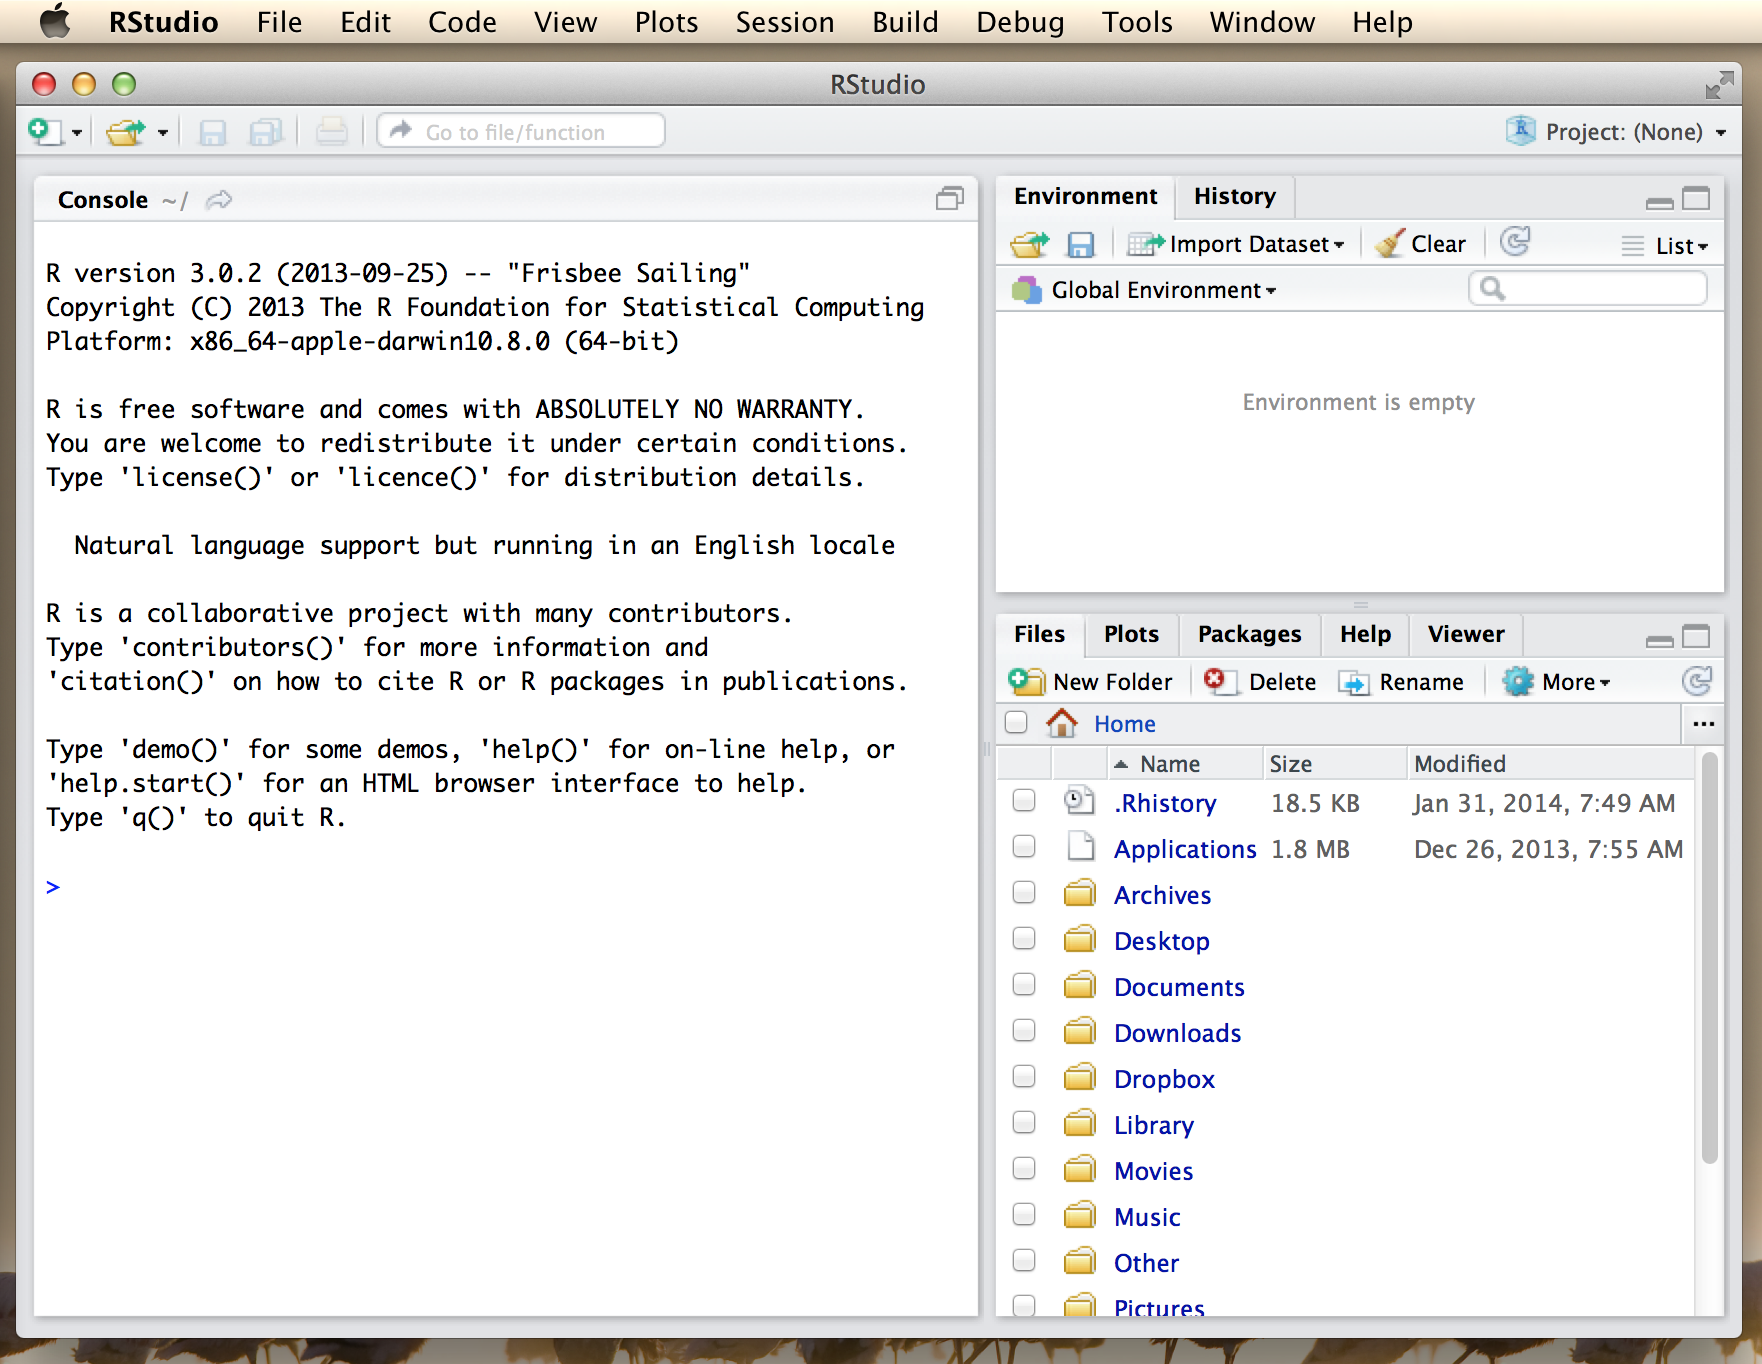
\epsfig{file = ../img/introR/Rstudio2.eps,clip=true, width = 14cm}
\caption{An R session in progress running through Rstudio. The picture shows Rstudio running on a Mac, but the Windows interface is almost identical.}
\label{fig:rstudio}
\HR
\end{center}
\end{figure}

Once it's finished downloading, open the installer file in the usual way to install Rstudio. After it's finished installing, you can start \R\ by opening Rstudio.  You don't need to open R.app or R.exe in order to access \R. Rstudio will take care of that for you. To illustrate what Rstudio looks like, Figure~\ref{fig:rstudio} shows a screenshot of an \R\ session in progress. In this screenshot, you can see that it's running on a Mac, but it looks almost identical no matter what operating system you have. The Windows version looks more like a Windows application (e.g., the menus are attached to the application window and the colour scheme is slightly different), but it's more or less identical. There are a few minor differences in where things are located in the menus (I'll point them out as we go along) and in the shortcut keys, because Rstudio is trying to ``feel'' like a proper Mac application or a proper Windows application, and this means that it has to change its behaviour a little bit depending on what computer it's running on. Even so, these differences are very small: I started out using the Mac version of Rstudio and then started using the Windows version as well in order to write these notes.

The only ``shortcoming'' I've found with Rstudio is that -- as of this writing -- it's still a work in progress. The current version as I type this is 0.98.501, which means that it's in beta testing (the official release is version 1.0). Even so, I think that the beta version of Rstudio provides a better user experience than anything else I've tried: it really is the best option available in my opinion. The ``problem'' is that they keep improving it. New features keep turning up the more recent releases, so there's a good chance that by the time you read this book there will be a version out that has some really neat things that weren't in the version that I'm using now.

\SUBSECTION{Starting up \R~\label{sec:startingR}}

One way or another, regardless of what operating system you're using and regardless of whether you're using Rstudio, or the default GUI, or even the command line, it's time to open \R\ and get started. When you do that, the first thing you'll see (assuming that you're looking at the \keyterm{\R\ console}, that is) is a whole lot of text that doesn't make much sense. It should look something like this:
\begin{rblock}
R version 3.0.2 (2013-09-25) -- "Frisbee Sailing"
Copyright (C) 2013 The R Foundation for Statistical Computing
Platform: x86_64-apple-darwin10.8.0 (64-bit)

R is free software and comes with ABSOLUTELY NO WARRANTY.
You are welcome to redistribute it under certain conditions.
Type 'license()' or 'licence()' for distribution details.

  Natural language support but running in an English locale

R is a collaborative project with many contributors.
Type 'contributors()' for more information and
'citation()' on how to cite R or R packages in publications.

Type 'demo()' for some demos, 'help()' for on-line help, or
'help.start()' for an HTML browser interface to help.
Type 'q()' to quit R.

> 
\end{rblock}
Most of this text is pretty uninteresting, and when doing real data analysis you'll never really pay much attention to it. The important part of it is this...
\begin{rblock}
> 
\end{rblock}
... which has a flashing cursor next to it. That's the \keyterm{command prompt}. When you see this, it means that \R\ is waiting patiently for you to do something! 


\section{Typing commands at the \R\ console\label{sec:firstcommand}}


One of the easiest things you can do with \R\ is use it as a simple calculator, so it's a good place to start. For instance, try typing \rtext{10 + 20}, and hitting enter.\FOOTNOTE{Seriously. If you're in a position to do so, open up \R\ and start typing. The simple act of typing it rather than ``just reading'' makes a big difference. It makes the concepts more concrete, and it ties the abstract ideas (programming and statistics) to the actual context in which you need to use them. Statistics is something you {\it do}, not just something you read about in a textbook.} When you do this, you've entered a \keyterm{command}, and \R\ will ``execute'' that command. What you see on screen now will be this:
\begin{rblock1}
> @usr{10 + 20}
[1] 30
\end{rblock1}
Not a lot of surprises in this extract. But there's a few things worth talking about, even with such a simple example. Firstly, it's important that you understand how to read the extract. In this example, what {\it I} typed was the \rtext{10 + 20} part. I didn't type the \rtextoutput{>} symbol: that's just the \R\ command prompt and isn't part of the actual command. And neither did I type the \rtextoutput{[1] 30} part. That's what \R\ printed out in response to my command. 

Secondly, it's important to understand how the output is formatted. Obviously, the correct answer to the sum \rtext{10 + 20} is \rtextoutput{30}, and not surprisingly \R\ has printed that out as part of its response. But it's also printed out this \rtextoutput{[1]} part, which probably doesn't make a lot of sense to you right now. You're going to see that a lot. I'll talk about what this means in a bit more detail later on, but for now you can think of \rtextoutput{[1] 30} as if \R\ were saying ``the answer to the 1st question you asked is 30''. That's not quite the truth, but it's close enough for now. And in any case it's not really very interesting at the moment: we only asked \R\ to calculate one thing, so obviously there's only one answer printed on the screen. Later on this will change, and the \rtextoutput{[1]} part will start to make a bit more sense. For now, I just don't want you to get confused or concerned by it. 

\SUBSECTION{Be very careful to avoid typos}

Before we go on to talk about other types of calculations that we can do with \R, there's a few other things I want to point out. The first thing is that, while \R\ is good software, it's still software. It's pretty stupid, and because it's stupid it can't handle typos. It takes it on faith that you meant to type {\it exactly} what you did type. For example, suppose that you forgot to hit the shift key when trying to type \rtext{+}, and as a result your command ended up being \rtext{10 = 20} rather than \rtext{10 + 20}. Here's what happens:
\begin{rblock1}
> @usr{10 = 20}
Error in 10 = 20 : invalid (do_set) left-hand side to assignment
\end{rblock1}
What's happened here is that \R\ has attempted to interpret \rtext{10 = 20} as a command, and spits out an error message because the command doesn't make any sense to it. When a {\it human} looks at this, and then looks down at his or her keyboard and sees that \rtext{+} and \rtext{=} are on the same key, it's pretty obvious that the command was a typo. But \R\ doesn't know this, so it gets upset. And, if you look at it from its perspective, this makes sense. All that \R\ ``knows'' is that \rtext{10} is a legitimate number, \rtext{20} is a legitimate number, and \rtext{=} is a legitimate part of the language too. In other words, from its perspective this really does look like the user meant to type \rtext{10 = 20}, since all the individual parts of that statement are legitimate and it's too stupid to realise that this is probably a typo. Therefore, \R\ takes it on faith that this is exactly what you meant... it only ``discovers'' that the command is nonsense when it tries to follow your instructions, typo and all. And then it whinges, and spits out an error.

Even more subtle is the fact that some typos won't produce errors at all, because they happen to correspond to ``well-formed'' \R\ commands. For instance, suppose that not only did I forget to hit the shift key when trying to type \rtext{10 + 20}, I also managed to press the key next to one I meant do. The resulting typo would produce the command \rtext{10 - 20}. Clearly, \R\ has no way of knowing that you meant to {\it add} 20 to 10, not {\it subtract} 20 from 10, so what happens this time is this:
\begin{rblock1}
> @usr{10 - 20}
[1] -10
\end{rblock1}
In this case, \R\ produces the right answer, but to the the wrong question. 

To some extent, I'm stating the obvious here, but it's important. The people who wrote \R\ are smart. You, the user, are smart. But \R\ itself is dumb. And because it's dumb, it has to be mindlessly obedient. It does {\it exactly} what you ask it to do. There is  no equivalent to ``autocorrect'' in \R, and for good reason. When doing advanced stuff -- and even the simplest of statistics is pretty advanced in a lot of ways -- it's dangerous to let a mindless automaton like \R\ try to overrule the human user. But because of this, it's your responsibility to be careful. Always make sure you type {\it exactly what you mean}. When dealing with computers, it's not enough to type ``approximately'' the right thing. In general, you absolutely {\it must} be precise in what you say to \R\ ... like all machines it is too stupid to be anything other than absurdly literal in its interpretation.

\SUBSECTION{\R\ is (a bit) flexible with spacing}

Of course, now that I've been so uptight about the importance of always being precise, I should point out that there are some exceptions. Or, more accurately, there are some situations in which \R\ does show a bit more flexibility than my previous description suggests. The first thing \R\ is smart enough to do is ignore redundant spacing. What I mean by this is that, when I typed \rtext{10 + 20} before, I could equally have done this
\begin{rblock1}
> @usr{10    + 20}
[1] 30
\end{rblock1}
or this 
\begin{rblock1}
> @usr{10+20}
[1] 30
\end{rblock1}
and I would get exactly the same answer. However, that doesn't mean that you can insert spaces in any old place. When we looked at the startup documentation in Section~\ref{sec:startingR} it suggested that you could type \rtext{citation()} to get some information about how to cite \R. If I do so...
\begin{rblock2}
> #usr[citation()]
To cite R in publications use:

  R Core Team (2013). R: A language and environment
  for statistical computing. R Foundation for
  Statistical Computing, Vienna, Austria. URL
  http://www.R-project.org/.

BLAH BLAH BLAH

We have invested a lot of time and effort in creating
R, please cite it when using it for data analysis. See
also ?citation("pkgname")? for citing R packages.
\end{rblock2}
... it tells me to cite the \R\ manual \cite{R2013}. Obviously, the \rtextoutput{BLAH BLAH BLAH} part isn't actually part of what \R\ prints out: when you see that it means that I've chopped out some parts of the output that I don't think are very interesting or relevant. I'll do that a lot. Anyway, getting back to my original point, let's see what happens when I try changing the spacing. If I insert spaces in between the word and the parentheses, or inside the parentheses themselves, then all is well. That is, either of these two commands
\begin{rblock1}
> @usr{citation ()}
> @usr{citation(  )}
\end{rblock1}
will produce exactly the same response. However, what I can't do is insert spaces in the middle of the word. If I try to do this, \R\ gets upset:
\begin{rblock1}
> @usr{citat ion()}
Error: unexpected symbol in "citat ion"
\end{rblock1}
Throughout this book I'll vary the way I use spacing a little bit, just to give you a feel for the different ways in which spacing can be used. I'll try not to do it too much though, since it's generally considered to be good practice to be consistent in how you format your commands. 

\SUBSECTION{\R\ can sometimes tell that you're not finished yet (but not often)}

One more thing I should point out. If you hit enter in a situation where it's ``obvious'' to \R\ that you haven't actually finished typing the command, \R\ is just smart enough to keep waiting. For example, if you type \rtext{10 + } and then press enter, even \R\ is smart enough to realise that you probably wanted to type in another number. So here's what happens:
\begin{rblock1}
> @usr{10+}
+ 
\end{rblock1}
and there's a blinking cursor next to the plus sign. What this means is that \R\ is still waiting for you to finish. It ``thinks'' you're still typing your command, so it hasn't tried to execute it yet. In other words, this plus sign is actually another command prompt. It's different from the usual one (i.e., the \rtextoutput{>} symbol) to remind you that \R\ is going to ``add'' whatever you type now to what you typed last time. For example, if I then go on to type \rtext{3} and hit enter, what I get is this:
\begin{rblock1}
> @usr{10+}
+ @usr{20}
[1] 30
\end{rblock1}
And as far as \R\ is concerned, this is {\it exactly} the same as if you had typed \rtext{10 + 20}. Similarly, consider the \rtext{citation()} command that we talked about in the previous section. Suppose you hit enter after typing \rtext{citation(}. Once again, \R\ is smart enough to realise that there must be more coming -- since you need to add the \rtext{)} character --  so it waits. I can even hit enter several times and it will keep waiting: 
\begin{rblock1}
> @usr{citation(}
+ 
+ 
+ @usr{)}
\end{rblock1}
I'll make use of this a lot in this book. A lot of the commands that we'll have to type are pretty long, and they're visually a bit easier to read if I break it up over several lines. If you start doing this yourself, you'll eventually get yourself in trouble (it happens to us all). Maybe you start typing a command, and then you realise you've screwed up. For example,
\begin{rblock1}
> @usr{citblation( }
+ 
+ 
\end{rblock1}
You'd probably prefer \R\ not to try running this command, right? If you want to get out of this situation, just hit the `escape' key.\FOOTNOTE{If you're running R from the terminal rather than from Rstudio, escape doesn't work: use CTRL-C instead.} \R\ will return you to the normal command prompt (i.e. \rtext{>}) {\it without} attempting to execute the botched command.


That being said, it's not often the case that \R\ is smart enough to tell that there's more coming.
For instance, in the same way that I can't add a space in the middle of a word, I can't hit enter in the middle of a word either. If I hit enter after typing \rtext{citat} I get an error, because \R\ thinks I'm interested in an ``object'' called \rtext{citat} and can't find it:
\begin{rblock1}
> @usr{citat}
Error: object 'citat' not found
\end{rblock1}
What about if I typed \rtext{citation} and hit enter? In this case we get something very odd, something that we definitely {\it don't} want, at least at this stage. Here's what happens:
\begin{rblock2}
> #usr[citation]
function (package = "base", lib.loc = NULL, auto = NULL) 
{
    dir <- system.file(package = package, lib.loc = lib.loc)
    if (dir == "") 
        stop(gettextf("package '%s' not found", package), domain = NA)

BLAH BLAH BLAH
\end{rblock2}
where the \rtextoutput{BLAH BLAH BLAH} goes on for rather a long time, and you don't know enough \R\ yet to understand what all this gibberish actually means. This incomprehensible output can be quite intimidating to novice users, and unfortunately it's very easy to forget to type the parentheses; so almost certainly you'll do this by accident. Do not panic when this happens. Simply ignore the gibberish.  As you become more experienced this gibberish will start to make sense, and you'll find it quite handy to print this stuff out.\FOOTNOTE{For advanced users: yes, as you've probably guessed, \R\ is printing out the source code for the function.}  But for now just try to remember to add the parentheses when typing your commands.

\section{Doing simple calculations with \R~\label{sec:arithmetic}}

Okay, now that we've discussed some of the tedious details associated with typing \R\ commands, let's get back to learning how to use the most powerful piece of statistical software in the world as a \$2 calculator. So far, all we know how to do is addition. Clearly, a calculator that only did addition would be a bit stupid, so I should tell you about how to perform other simple calculations using \R. But first, some more terminology. Addition is an example of an ``operation'' that you can perform (specifically, an arithmetic operation), and the \keyterm{operator} that performs it is \rtext{+}. To people with a programming or mathematics background, this terminology probably feels pretty natural, but to other people it might feel like I'm trying to make something very simple (addition) sound more complicated than it is (by calling it an arithmetic operation). To some extent, that's true: if addition was the only operation that we were interested in, it'd be a bit silly to introduce all this extra terminology. However, as we go along, we'll start using more and more different kinds of operations, so it's probably a good idea to get the language straight now, while we're still talking about very familiar concepts like addition! 

\SUBSECTION{Adding, subtracting, multiplying and dividing}

%\index{R}{{+}}
%\index{R}{{-}}
%\index{R}{{*}}
%\index{R}{{/}}

\begin{table}
\begin{center}
\caption{Basic arithmetic operations in \R. These five operators are used very frequently throughout the text, so it's important to be familiar with them at the outset. There are others as well, which I'll discuss in Chapter~\ref{ch:datahandling}.}
\tabcapsep
\label{tab:arithmetic1}
\begin{tabular}{lc|cc} 
operation  		& operator 	& example input & example output\\ \hline
addition			&\rtext{+}	& \rtext{10 + 2}	& \rtextoutput{12}\\
subtraction		&\rtext{-}	& \rtext{9 - 3} 	& \rtextoutput{6} \\
multiplication	&\rtext{*}	& \rtext{5 * 5} 	& \rtextoutput{25}\\ 
division			&\rtext{/}	& \rtext{10 / 3} & \rtextoutput{3}\\ 
power	& \rtextverb#^#	& \rtext{5} \rtextverb#^# \rtext{2}& \rtextoutput{25} \\
\end{tabular} \tabcapsep
\HR
\end{center}
\end{table}

So, now that we have the terminology, let's learn how to perform some arithmetic operations in \R. To that end, Table~\ref{tab:arithmetic1} lists the operators that correspond to the basic arithmetic we learned in primary school: addition, subtraction, multiplication and division. As you can see, \R\ uses fairly standard symbols to denote each of the different operations you might want to perform: addition is done using the \rtext{+} operator, subtraction is performed by the \rtext{-} operator, and so on. So if I wanted to find out what 57 times 61 is (and who wouldn't?), I can use \R\ instead of a calculator, like so:
\begin{rblock1}
> @usr{57 * 61}
[1] 3477
\end{rblock1}
So that's handy. 


\SUBSECTION{Taking powers}


The first four operations listed in Table~\ref{tab:arithmetic1} are things we all learned in primary school, but they aren't the only arithmetic operations built into \R. There are three other arithmetic operations that I should probably mention: taking powers, doing integer division, and calculating a modulus. Of the three, the only one that is of any real importance for the purposes of this book is taking powers, so I'll discuss that one here: the other two are discussed in Chapter~\ref{ch:datahandling}.

For those of you who can still remember your high school maths, this should be familiar. But for some people high school maths was a long time ago, and others of us didn't listen very hard in high school. It's not complicated. As I'm sure everyone will probably remember the moment they read this, the act of multiplying a number $x$ by itself $n$ times is called ``raising $x$ to the $n$-th power''. Mathematically, this is written as $x^n$. Some values of $n$ have special names: in particular $x^2$ is called $x$-squared, and $x^3$ is called $x$-cubed. So, the 4th power of 5 is calculated like this:
$$
5^4 = 5 \times 5 \times 5 \times 5 
$$
One way that we could calculate $5^4$ in \R\ would be to type in the complete multiplication as it is shown in the equation above. That is, we could do this
\begin{rblock1}
> @usr{5 * 5 * 5 * 5}
[1] 625
\end{rblock1}
but it does seem a bit tedious. It would be very annoying indeed if you wanted to calculate $5^{15}$, since the command would end up being quite long. Therefore, to make our lives easier, we use the power operator instead. When we do that, our command to calculate $5^4$ goes like this:
\begin{rblock1}
> @usr{5 ^ 4}
[1] 625
\end{rblock1}
Much easier.


\SUBSECTION{Doing calculations in the right order\label{sec:bedmas}}

Okay. At this point, you know how to take one of the most powerful pieces of statistical software in the world, and use it as a \$2 calculator. And as a bonus, you've learned a few very basic programming concepts. That's not nothing (you could argue that you've just saved yourself \$2) but on the other hand, it's not very much either. In order to use \R\ more effectively, we need to introduce more programming concepts.

In most situations where you would want to use a calculator, you might want to do multiple calculations. \R\ lets you do this, just by typing in longer commands. \marginpar{If you're reading this with \R\ open, a good learning trick is to try typing in a few different variations on what I've done here. If you experiment with your commands, you'll quickly learn what works and what doesn't} In fact, we've already seen an example of this earlier, when I typed in \rtext{5 * 5 * 5 * 5}. However, let's try a slightly different example:
\begin{rblock1}
> @usr{1 + 2 * 4}
[1] 9
\end{rblock1}
Clearly, this isn't a problem for \R\ either. However, it's worth stopping for a second, and thinking about what \R\ just did. Clearly, since it gave us an answer of \rtextoutput{9} it must have multiplied \rtext{2 * 4} (to get an interim answer of 8) and then added 1 to that. But, suppose it had decided to just go from left to right: if \R\ had decided instead to add \rtext{1+2} (to get an interim answer of 3) and then multiplied by 4, it would have come up with an answer of \rtextoutput{12}. 

To answer this, you need to know the \keyterm{order of operations} that \R\ uses. If you remember back to your high school maths classes, it's actually the same order that you got taught when you were at school: the ``\textsc{bedmas}'' order.\FOOTNOTE{For advanced users: if you want a table showing the complete order of operator precedence in \R, type \rtextsmall{?Syntax}. I haven't included it in this book since there are quite a few different operators, and we don't need that much detail. Besides, in practice most people seem to figure it out from seeing examples: until writing this book I never looked at the formal statement of operator precedence for any language I ever coded in, and never ran into any difficulties.} That is, first calculate things inside {\bf B}rackets \rtext{()}, then calculate {\bf E}xponents \rtextverb#^#, then {\bf D}ivision \rtext{/} and {\bf M}ultiplication \rtext{*}, then {\bf A}ddition \rtext{+} and {\bf S}ubtraction \rtext{-}. So, to continue the example above, if we want to force \R\ to calculate the \rtext{1+2} part before the multiplication, all we would have to do is enclose it in brackets:
\begin{rblock1}
> @usr{(1 + 2) * 4} 
[1] 12
\end{rblock1}
This is a fairly useful thing to be able to do. The only other thing I should point out about order of operations is what to expect when you have two operations that have the same priority: that is, how does \R\ resolve ties? For instance, multiplication and division are actually the same priority, but what should we expect when we give \R\ a problem like \rtext{4 / 2 * 3} to solve? If it evaluates the multiplication first and then the division, it would calculate a value of two-thirds. But if it evaluates the division first it calculates a value of 6. The answer, in this case, is that \R\ goes from {\it left to right}, so in this case the division step would come first:
\begin{rblock1}
> @usr{4 / 2 * 3} 
[1] 6
\end{rblock1}

All of the above being said, it's helpful to remember that {\it brackets always come first}. So, if you're ever unsure about what order \R\ will do things in, an easy solution is to enclose the thing {\it you} want it to do first in brackets.  There's nothing stopping you from typing \rtext{(4 / 2) * 3}. By enclosing the division in brackets we make it clear which thing is supposed to happen first. In this instance you wouldn't have needed to, since \R\ would have done the division first anyway, but when you're first starting out it's better to make sure \R\ does what you want!



\section{Storing a number as a variable~\label{sec:assign}}
%\index{R}{{<-}}
%\index{R}{{=}}

One of the most important things to be able to do in \R\ (or any programming language, for that matter) is to store information in \keyterm{variables}. Variables in \R\ aren't exactly the same thing as the variables we talked about in the last chapter on research methods, but they are similar. At a conceptual level you can think of a variable as {\it label} for a certain piece of information, or even several different pieces of information. When doing statistical analysis in \R\ all of your data (the variables you measured in your study) will be stored as variables in \R, but as well see later in the book you'll find that you end up creating variables for other things too. However, before we delve into all the messy details of data sets and statistical analysis, let's look at the very basics for how we create variables and work with them. 

\SUBSECTION{Variable assignment using \rtext{<-} and \rtext{->}}

Since we've been working with numbers so far, let's start by creating variables to store our numbers. And since most people like concrete examples, let's invent one. Suppose I'm trying to calculate how much money I'm going to make from this book. There's several different numbers I might want to store. Firstly, I need to figure out how many copies I'll sell. This isn't exactly {\it Harry Potter}, so let's assume I'm only going to sell one copy per student in my class. That's 350 sales, so let's create a variable called \rtext{sales}. What I want to do is assign a \keyterm{value} to my variable \rtext{sales}, and that value should be \rtext{350}. We do this by using the \keyterm{assignment operator}, which is \rtext{<-}. Here's how we do it:
\begin{rblock1}
> @usr{sales <- 350}
\end{rblock1}
When you hit enter, \R\ doesn't print out any output.\FOOTNOTE{If you are using Rstudio, and the ``environment'' panel (formerly known as the ``workspace'' panel) is visible when you typed the command, then you probably saw something happening there. That's to be expected, and is quite helpful. However, there's two things to note here (1) I haven't yet explained what that panel does, so for now just ignore it, and (2) this is one of the helpful things Rstudio does, not a part of \R\ itself.} It just gives you another command prompt. However, behind the scenes \R\ has created a variable called \rtext{sales} and given it a value of \rtext{350}. You can check that this has happened by asking \R\ to print the variable on screen. And the simplest way to do {\it that} is to type the name of the variable and hit enter\FOOTNOTE{As we'll discuss later, by doing this we are implicitly using the \rtextsmall{print()} function.}
\begin{rblock1}
> @usr{sales}
[1] 350
\end{rblock1}
So that's nice to know. Anytime you can't remember what \R\ has got stored in a particular variable, you can just type the name of the variable and hit enter. 

Okay, so now we know how to assign variables. Actually, there's a bit more you should know. Firstly, one of the curious features of \R\ is that there are several different ways of making assignments. In addition to the \rtext{<-} operator, we can also use \rtext{->} and \rtext{=}, and it's pretty important to understand the differences between them.\FOOTNOTE{Actually, in keeping with the \R\ tradition of providing you with a billion different screwdrivers (even when you're actually looking for a hammer) these aren't the only options. There's also the \rtextsmall{assign()} function, and the \rtextsmall{<<-} and \rtextsmall{->>} operators. However, we won't be using these at all in this book.} Let's start by considering \rtext{->}, since that's the easy one (we'll discuss the use of \rtext{=} in Section~\ref{sec:functionarguments}). As you might expect from just looking at the symbol, it's almost identical to \rtext{<-}. It's just that the arrow (i.e., the assignment) goes from left to right. So if I wanted to define my \rtext{sales} variable using \rtext{->}, I would write it like this:
\begin{rblock1}
> @usr{350 -> sales}
\end{rblock1}
This has the same effect: and it {\it still} means that I'm only going to sell \rtextoutput{350} copies. Sigh. Apart from this superficial difference, \rtext{<-} and \rtext{->} are identical. In fact, as far as \R\ is concerned, they're actually the same operator, just in a ``left form'' and a ``right form''.\FOOTNOTE{A quick reminder: when using operators like \rtextsmall{<-} and \rtextsmall{->} that span multiple characters, you can't insert spaces in the middle. That is, if you type \rtextsmall{- >} or \rtextsmall{< -}, \R\ will interpret your command the wrong way. And I will cry.}


\SUBSECTION{Doing calculations using variables}

Okay, let's get back to my original story. In my quest to become rich, I've written this textbook. To figure out how good a strategy is, I've started creating some variables in \R. In addition to defining a \rtext{sales} variable that counts the number of copies I'm going to sell, I can also create a variable called \rtext{royalty}, indicating how much money I get per copy. Let's say that my royalties are about \$7 per book:
\begin{rblock1}
> @usr{sales <- 350}
> @usr{royalty <- 7}
\end{rblock1}
The nice thing about variables (in fact, the whole point of having variables) is that we can do anything with a variable that we ought to be able to do with the information that it stores. That is, since \R\ allows me to multiply \rtext{350} by \rtext{7}
\begin{rblock1}
> @usr{350 * 7}
[1] 2450
\end{rblock1}
it also allows me to multiply \rtext{sales} by \rtext{royalty}
\begin{rblock1}
> @usr{sales * royalty}
[1] 2450
\end{rblock1}
As far as \R\ is concerned, the \rtext{sales * royalty} command is the same as the \rtext{350 * 7} command. Not surprisingly, I can assign the output of this calculation to a new variable, which I'll call \rtext{revenue}. And when we do this, the new variable \rtext{revenue} gets the value \rtext{2450}. So let's do that, and then get \R\ to print out the value of \rtext{revenue} so that we can verify that it's done what we asked:
\begin{rblock1}
> @usr{revenue <- sales * royalty}
> @usr{revenue}
[1] 2450
\end{rblock1}
That's fairly straightforward. A slightly more subtle thing we can do is reassign the value of my variable, based on its current value. For instance, suppose that one of my students (no doubt under the influence of psychotropic drugs) loves the book so much that he or she donates me an extra \$550. The simplest way to capture this is by a command like this:
\begin{rblock1}
> @usr{revenue <- revenue + 550}
> @usr{revenue}
[1] 3000
\end{rblock1}
In this calculation, \R\ has taken the old value of \rtext{revenue} (i.e., 2450) and added 550 to that value, producing a value of 3000. This new value is assigned to the \rtext{revenue} variable, overwriting its previous value. In any case, we now know that I'm expecting to make \$3000 off this. Pretty sweet, I thinks to myself. Or at least, that's what I thinks until I do a few more calculation and work out what the implied hourly wage I'm making off this looks like. 

\SUBSECTION{Rules and conventions for naming variables}

In the examples that we've seen so far, my variable names (\rtext{sales} and \rtext{revenue}) have just been English-language words written using lowercase letters. However, \R\ allows a lot more flexibility when it comes to naming your variables, as the following list of rules\FOOTNOTE{Actually, you can override any of these rules if you want to, and quite easily. All you have to do is add quote marks or backticks around your non-standard variable name. For instance \rtextsmall{`) my sales>` <- 350} would work just fine, but it's almost never a good idea to do this.} illustrates:

\begin{itemize}
\item Variable names can only use the upper case alphabetic characters \rtext{A}-\rtext{Z} as well as the lower case characters \rtext{a}-{\rtext{z}}. You can also include numeric characters \rtext{0}-\rtext{9} in the variable name, as well as the period \rtext{.} or underscore \rtextverb#_# character. In other words, you can use \rtextverb#SaL.e_s# as a variable name (though I can't think why you would want to), but you can't use \rtext{Sales?}. 
\item Variable names cannot include spaces: therefore \rtext{my sales} is not a valid name, but \rtext{my.sales} is.
\item Variable names are case sensitive: that is, \rtext{Sales} and \rtext{sales} are {\it different} variable names.
\item Variable names must start with a letter or a period. You can't use something like \rtextverb#_sales# or \rtext{1sales} as a variable name. You can use \rtext{.sales} as a variable name if you want, but it's not usually a good idea. By convention, variables starting with a \rtext{.} are used for special purposes, so you should avoid doing so. 
\item Variable names cannot be one of the reserved keywords. These are special names that \R\ needs to keep ``safe'' from us mere users, so you can't use them as the names of variables. The keywords are: \rtext{if}, \rtext{else}, \rtext{repeat}, \rtext{while}, \rtext{function}, \rtext{for}, \rtext{in}, \rtext{next}, \rtext{break}, \rtext{TRUE}, \rtext{FALSE}, \rtext{NULL}, \rtext{Inf}, \rtext{NaN}, \rtext{NA}, \rtextverb#NA_integer_#, \rtextverb#NA_real_#, \rtextverb#NA_complex_#, and finally,  \rtextverb#NA_character_#. Don't feel especially obliged to memorise these: if you make a mistake and try to use one of the keywords as a variable name, \R\ will complain about it like the whiny little automaton it is.
\end{itemize}

\noindent
In addition to those rules that \R\ enforces, there are some informal conventions that people tend to follow when naming variables. One of them you've already seen: i.e., don't use variables that start with a period. But there are several others. You aren't obliged to follow these conventions, and there are many situations in which it's advisable to ignore them, but it's generally a good idea to follow them when you can:

\begin{itemize}
\item Use informative variable names. As a general rule, using meaningful names like \rtext{sales} and \rtext{revenue} is preferred over arbitrary ones like \rtext{variable1} and \rtext{variable2}. Otherwise it's very hard to remember what the contents of different variables are, and it becomes hard to understand what your commands actually do. 
\item Use short variable names. Typing is a pain and no-one likes doing it. So we much prefer to use a name like \rtext{sales} over a name like \rtext{sales.for.this.book.that.you.are.reading}. Obviously there's a bit of a tension between using informative names (which tend to be long) and using short names (which tend to be meaningless), so use a bit of common sense when trading off these two conventions.
\item Use one of the conventional naming styles for multi-word variable names. Suppose I want to name a variable that stores ``my new salary''. Obviously I can't include spaces in the variable name, so how should I do this? There are three different conventions that you sometimes see \R\ users employing. Firstly, you can separate the words using periods, which would give you \rtextverb#my.new.salary# as the variable name. Alternatively, you could separate words using underscores, as in \rtextverb#my_new_salary#. Finally, you could use capital letters at the beginning of each word (except the first one), which gives you \rtext{myNewSalary} as the variable name. I don't think there's any strong reason to prefer one over the other,\FOOTNOTE{For very advanced users: there is one exception to this. If you're naming a function, don't use \rtextsmall{.} in the name unless you are intending to make use of the S3 object oriented programming system in \R. If you don't know what S3 is, then you definitely don't want to be using it! For function naming, there's been a trend among \R\ users to prefer \rtextsmall{myFunctionName}.} but it's important to be consistent.
\end{itemize}




\section{Using functions to do calculations\label{sec:usingfunctions}}

The symbols \rtext{+}, \rtext{-}, \rtext{*} and so on are examples of operators. As we've seen, you can do quite a lot of calculations just by using these operators. However, in order to do more advanced calculations (and later on, to do actual statistics), you're going to need to start using \keyterm{functions}.\FOOTNOTE{A side note for students with a programming background. Technically speaking, operators {\it are} functions in \R: the addition operator \rtextsmall{+} is actually a convenient way of calling the addition function \rtextsmall{`+`()}. Thus \rtextsmall{10+20} is equivalent to the function call \rtextsmall{`+`(20, 30)}. Not surprisingly, no-one ever uses this version. Because that would be stupid.} I'll talk in more detail about functions and how they work in Section~\ref{sec:functions}, but for now let's just dive in and use a few. To get started, suppose I wanted to take the square root of 225. The  square root, in case your high school maths is a bit rusty, is just the opposite of squaring a number. So, for instance, since ``5 squared is 25'' I can say that ``5 is the square root of 25''. The usual notation for this is 
$$
\sqrt{25} = 5
$$
though sometimes you'll also see it written like this
$
25^{0.5} = 5.
$
This second way of writing it is kind of useful to ``remind'' you of the mathematical fact that ``square root of $x$'' is actually the same as ``raising $x$ to the power of 0.5''. Personally, I've never found this to be terribly meaningful psychologically, though I have to admit it's quite convenient mathematically. Anyway, it's not important. What is important is that you remember what a square root is, since we're going to need it later on.

To calculate the square root of 25, I can do it in my head pretty easily, since I memorised my multiplication tables when I was a kid. It gets harder when the numbers get bigger, and pretty much impossible if they're not whole numbers. This is where something like \R\ comes in very handy. Let's say I wanted to calculate $\sqrt{225}$, the square root of 225. There's two ways I could do this using \R. Firstly, since the square root of 255 is the same thing as raising 225 to the power of 0.5, I could use the power operator \rtextverb#^#, just like we did earlier:
\begin{rblock1}
> @usr{225 ^ 0.5}
[1] 15
\end{rblock1}
However, there's a second way that we can do this, since \R\ also provides a \keyterm{square root function}, \rtext{sqrt()}. To calculate the square root of 255 using this function, what I do is insert the number \rtext{225} in the parentheses. That is, the command I type is this:
%\index{R}{sqrt}
\begin{rblock1}
> @usr{sqrt( 225 )}
[1] 15
\end{rblock1}
and as you might expect from our previous discussion, the spaces in between the parentheses are purely cosmetic. I could have typed \rtext{sqrt(225)} or \rtext{sqrt( 225   )} and gotten the same result. When we use a function to do something, we generally refer to this as \keyterm{calling} the function, and the values that we type into the function (there can be more than one) are referred to as the \keyterm{arguments} of that function. 

Obviously, the \rtext{sqrt()} function doesn't really give us any new functionality, since we already knew how to do square root calculations by using the power operator \rtextverb#^#, though I do think it looks nicer when we use \rtext{sqrt()}. However, there are lots of other functions in \R: in fact, almost everything of interest that I'll talk about in this book is an \R\ function of some kind. For example, one function that we will need to use in this book is the \keyterm{absolute value function}. Compared to the square root function, it's extremely simple: it just converts negative numbers to positive numbers, and leaves positive numbers alone. Mathematically, the absolute value of $x$ is written $|x|$ or sometimes $\mbox{abs}(x)$. Calculating absolute values in \R\ is pretty easy, since \R\ provides the \rtext{abs()} function that you can use for this purpose. When you feed it a positive number...
\begin{rblock1}
> @usr{abs( 21 )}
[1] 21
\end{rblock1}
the absolute value function does nothing to it at all. But when you feed it a negative number, it spits out the positive version of the same number, like this:
\begin{rblock1} 
> @usr{abs( -13 )}
[1] 13
\end{rblock1} 
In all honesty, there's nothing that the absolute value function does that you couldn't do just by looking at the number and erasing the minus sign if there is one. However, there's a few places later in the book where we have to use absolute values, so I thought it might be a good idea to explain the meaning of the term early on.


%\SUBSECTION{Combining functions}

Before moving on, it's worth noting that -- in the same way that \R\ allows us to put multiple operations together into a longer command, like \rtext{1 + 2*4} for instance -- it also lets us put functions together and even combine functions with operators if we so desire. For example, the following is a perfectly legitimate command:
\begin{rblock1}
> @usr{sqrt( 1 + abs(-8) )}
[1] 3
\end{rblock1}
When \R\ executes this command, starts out by calculating the value of \rtext{abs(-8)}, which produces an intermediate value of \rtext{8}. Having done so, the command simplifies to \rtext{sqrt( 1 + 8 )}. To solve the square root\FOOTNOTE{A note for the mathematically inclined: \R\ does support complex numbers, but unless you explicitly specify that you want them it assumes all calculations must be real valued. By default, the square root of a negative number is treated as undefined: \rtextsmall{sqrt(-9)} will produce \rtextsmall{NaN} (not a number) as its output. To get complex numbers, you would type \rtextsmall{sqrt(-9+0i)}  and \R\ would now return \rtextsmall{0+3i}. However, since we won't have any need for complex numbers in this book, I won't refer to them again.} it first needs to add \rtext{1 + 8} to get \rtext{9}, at which point it evaluates \rtext{sqrt(9)}, and so it finally outputs a value of \rtextoutput{3}.



\SUBSECTION{Function arguments, their names and their defaults~\label{sec:functionarguments}}

There's two more fairly important things that you need to understand about how functions work in \R, and that's the use of ``named'' arguments, and 		default values'' for arguments. Not surprisingly, that's not to say that this is the last we'll hear about how functions work, but they are the last things we desperately need to discuss in order to get you started. To understand what these two concepts are all about, I'll introduce another function. The \rtext{round()} function can be used to round some value to the nearest whole number. For example, I could type this:
\begin{rblock1}
> @usr{round( 3.1415 )}
[1] 3
\end{rblock1}
Pretty straightforward, really. However, suppose I only wanted to round it to two decimal places: that is, I want to get \rtextoutput{3.14} as the output. The \rtext{round()} function supports this, by allowing you to input a second argument to the function that specifies the number of decimal places that you want to round the number to. In other words, I could do this: 
\begin{rblock1}
> @usr{round( 3.14165, 2 )}
[1] 3.14
\end{rblock1}
What's happening here is that I've specified {\it two} arguments: the first argument is the number that needs to be rounded (i.e., \rtext{3.1415}), the second argument is the number of decimal places that it should be rounded to (i.e., \rtext{2}), and the two arguments are separated by a comma. In this simple example, it's quite easy to remember which one argument comes first and which one comes second, but for more complicated functions this is not easy. Fortunately, most \R\ functions make use of \keyterm{argument names}. For the \rtext{round()} function, for example the number that needs to be rounded is specified using the \rtext{x} argument, and the number of decimal points that you want it rounded to is specified using the \rtext{digits} argument. Because we have these names available to us, we can specify the arguments to the function by name. We do so like this:
\begin{rblock1}
> @usr{round( x = 3.1415, digits = 2 )}
[1] 3.14
\end{rblock1}
Notice that this is kind of similar in spirit to variable assignment (Section~\ref{sec:assign}), except that I used \rtext{=} here, rather than \rtext{<-}. In both cases we're specifying specific values to be associated with a label. However, there are some differences between what I was doing earlier on when creating variables, and what I'm doing here when specifying arguments, and so as a consequence it's important that you use \rtext{=} in this context.


As you can see, specifying the arguments by name involves a lot more typing, but it's also a lot easier to read. Because of this, the commands in this book will usually specify arguments by name,\FOOTNOTE{The two functions discussed previously, \rtextsmall{sqrt()} and \rtextsmall{abs()}, both only have a single argument, \rtextsmall{x}. So I could have typed something like \rtextsmall{sqrt(x = 225)} or \rtextsmall{abs(x = -13)} earlier. The fact that all these functions use \rtextsmall{x} as the name of the argument that corresponds the ``main'' variable that you're working with is no coincidence. That's a fairly widely used convention. Quite often, the writers of \R\ functions will try to use conventional names like this to make your life easier. Or at least that's the theory. In practice it doesn't always work as well as you'd hope. } since that makes it clearer to you what I'm doing. However, one important thing to note is that when specifying the arguments using their names, it doesn't matter what order you type them in. But if you don't use the argument names, then you have to input the arguments in the correct order. In other words, these three commands all produce the same output...
\begin{rblock1}
> @usr{round( 3.14165, 2 )}
> @usr{round( x = 3.1415, digits = 2 )}
> @usr{round( digits = 2, x = 3.1415 )}
\end{rblock1}
but this one does not...
\begin{rblock1}
> @usr{round( 2, 3.14165 )}
\end{rblock1}
How do you find out what the correct order is? There's a few different ways, but the easiest one is to look at the help documentation for the function (see Section~\ref{sec:help}). However, if you're ever unsure, it's probably best to actually type in the argument name.

%\SUBSECTION{Default values~\label{sec:defaults}}

Okay, so that's the first thing I said you'd need to know: argument names. The second thing you need to know about is default values. Notice that the first time I called the \rtext{round()} function I didn't actually specify the \rtext{digits} argument at all, and yet \R\ somehow knew that this meant it should round to the nearest whole number. How did that happen? The answer is that the \rtext{digits} argument has a \keyterm{default value} of \rtext{0}, meaning that if you decide not to specify a value for \rtext{digits} then \R\ will act as if you had typed \rtext{digits = 0}. This is quite handy: the vast majority of the time when you want to round a number you want to round it to the nearest whole number, and it would be pretty annoying to have to specify the \rtext{digits} argument every single time. On the other hand, sometimes you actually do want to round to something other than the nearest whole number, and it would be even more annoying if \R\ didn't allow this! Thus, by having \rtext{digits = 0} as the default value, we get the best of both worlds.



\section{Letting Rstudio help you with your commands\label{sec:Rstudio1}}

Time for a bit of a digression. At this stage you know how to type in basic commands, including how to use \R\ functions. And it's probably beginning to dawn on you that there are a {\it lot} of \R\ functions, all of which have their own arguments. You're probably also worried that you're going to have to remember all of them! Thankfully, it's not that bad. In fact, very few data analysts bother to try to remember all the commands. What they really do is use tricks to make their lives easier. The first (and arguably most important one) is to use the internet. If you don't know how a particular \R\ function works, Google it. Second, you can look up the \R\ help documentation. I'll talk more about these two tricks in Section~\ref{sec:help}. But right now I want to call your attention to a couple of simple tricks that Rstudio makes available to you.

\SUBSECTION{Autocomplete using ``tab''}

The first thing I  want to call your attention to is the {\it autocomplete} ability in Rstudio.\FOOTNOTE{For advanced users:  obviously, this isn't just an Rstudio thing. If you're running R in a terminal window, tab autocomplete still works, and does so in exactly the way you'd expect. It's not as visually pretty as the Rstudio version, of course, and lacks some of the cooler features that Rstudio provides. I don't bother to document that here: my assumption is that if you are running \R\ in the terminal then you're already familiar with using tab autocomplete.}

Let's stick to our example above and assume that what you want to do is to round a number. This time around, start typing the name of the function that you want, and then hit the ``tab'' key. Rstudio will then display a little window like the one shown in Figure~\ref{fig:Rstudiotab}. In this figure, I've typed the letters \rtext{ro} at the command line, and then hit tab. The window has two panels. On the left, there's a list of variables and functions that start with the letters that I've typed shown in black text, and some grey text that tells you where that variable/function is stored. Ignore the grey text for now: it won't make much sense to you until we've talked about packages in Section~\ref{sec:packageinstall}. In Figure~\ref{fig:Rstudiotab} you can see that there's quite a few things that start with the letters \rtext{ro}: there's something called \rtext{rock}, something called \rtext{round}, something called \rtext{round.Date} and so on. The one we want is \rtext{round}, but if you're typing this yourself you'll notice that when you hit the tab key the window pops up with the top entry (i.e., \rtext{rock}) highlighted. You can use the up and down arrow keys to select the one that you want. Or, if none of the options look right to you, you can hit the escape key (``esc'') or the left arrow key to make the window go away. 

In our case, the thing we want is the \rtext{round} option, so we'll select that. When you do this, you'll see that the panel on the right changes. Previously, it had been telling us something about the \rtext{rock} data set (i.e., ``Measurements on 48 rock samples...'') that is distributed as part of \R. But when we select \rtext{round}, it displays information about the \rtext{round()} function, exactly as it is shown in Figure~\ref{fig:Rstudiotab}. This display is really handy. The very first thing it says is \texttt{round(x, digits = 0)}: what this is telling you is that the \rtext{round()} function has two arguments. The first argument is called \rtext{x}, and it doesn't have a default value. The second argument is \rtext{digits}, and it has a default value of 0. In a lot of situations, that's all the information you need. But Rstudio goes a bit further, and provides some additional information about the function underneath. Sometimes that additional information is very helpful, sometimes it's not: Rstudio pulls that text from the \R\ help documentation, and my experience is that the helpfulness of that documentation varies wildly. Anyway, if you've decided that \rtext{round()} is the function that you want to use, you can hit the right arrow or the enter key, and Rstudio will finish typing the rest of the function name for you. 

\begin{figure}[t]
\begin{center}
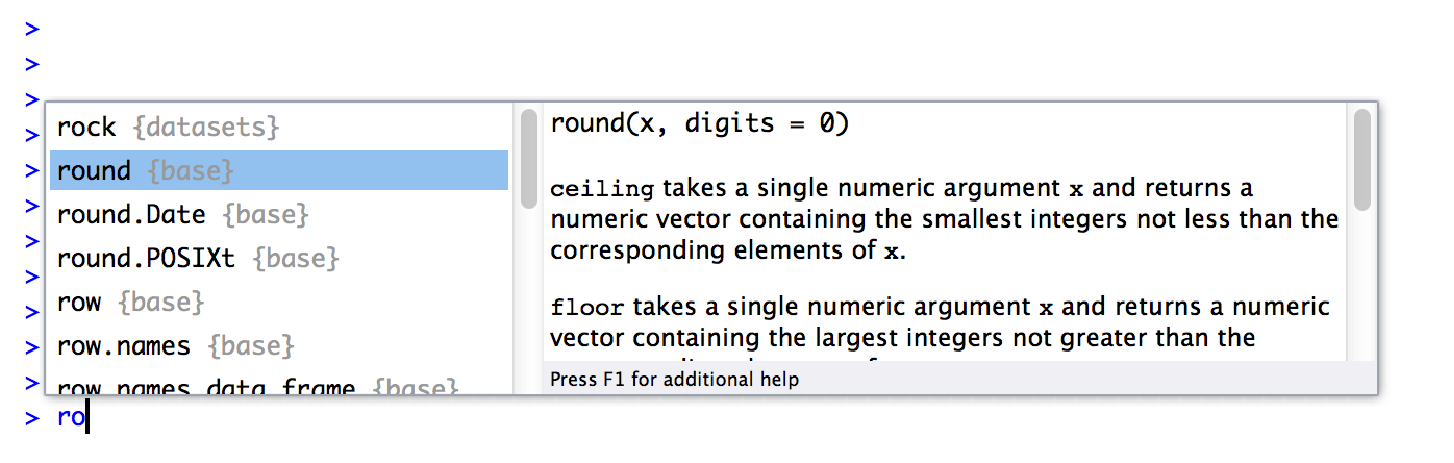
\epsfig{file=../img/introR/Rstudio_tab.eps,clip=true,width=14cm}
\caption{Start typing the name of a function or a variable, and hit the ``tab'' key. Rstudio brings up a little dialog box like this one that lets you select the one you want, and even prints out a little information about it.}
\HR
\label{fig:Rstudiotab}
\end{center}
\end{figure}

The Rstudio autocomplete tool works slightly differently if you've already got the name of the function typed and you're now trying to type the arguments. For instance, suppose I've typed \rtext{round(} into the console, and {\it then} I hit tab. Rstudio is smart enough to recognise that I already know the name of the function that I want, because I've already typed it! Instead, it figures that what I'm interested in is the {\it arguments} to that function. So that's what pops up in the little window. You can see this in Figure~\ref{fig:Rstudiotab2}. Again, the window has two panels, and you can interact with this window in exactly the same way that you did with the window shown in Figure~\ref{fig:Rstudiotab}. On the left hand panel, you can see a list of the argument names. On the right hand side, it displays some information about what the selected argument does. 


\begin{figure}[t]
\begin{center}
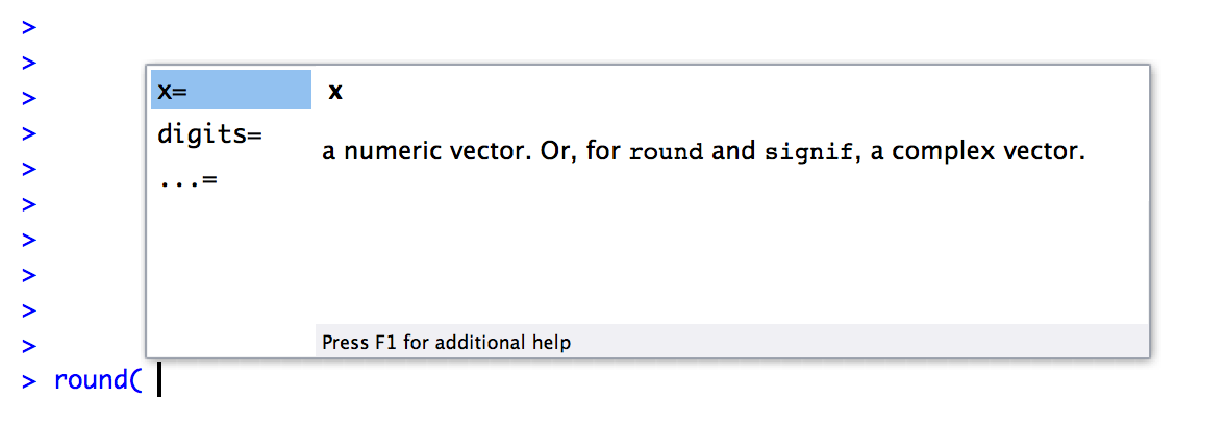
\epsfig{file=../img/introR/Rstudio_tab2.eps,clip=true,width=14cm}
\caption{If you've typed the name of a function already along with the left parenthesis and then hit the ``tab'' key, Rstudio brings up a different window to the one shown in Figure~\protect\ref{fig:Rstudiotab}. This one lists all the arguments to the function on the left, and information about each argument on the right.}
\HR
\label{fig:Rstudiotab2}
\end{center}
\end{figure}


\SUBSECTION{Browsing your command history}

One thing that \R\ does automatically is keep track of your ``command history''. That is, it remembers all the commands that you've previously typed. You can access this history in a few different ways. The simplest way is to use the up and down arrow keys. If you hit the up key, the \R\ console will show you the most recent command that you've typed. Hit it again, and it will show you the command before that. If you want the text on the screen to go away, hit escape\FOOTNOTE{Incidentally, that always works: if you've started typing a command and you want to clear it and start again, hit escape.} Using the up and down keys can be really handy if you've typed a long command that had one typo in it. Rather than having to type it all again from scratch, you can use the up key to bring up the command and fix it. 

The second way to get access to your command history is to look at the history panel in Rstudio. On the upper right hand side of the Rstudio window you'll see a tab labelled ``History''. Click on that, and you'll see a list of all your recent commands displayed in that panel: it should look something like Figure~\ref{fig:Rstudiohistory}. If you double click on one of the commands, it will be copied to the \R\ console. (You can achieve the same result by selecting the command you want with the mouse and then clicking the ``To Console'' button).\FOOTNOTE{Another method is to start typing some text and then hit the Control key and the up arrow together (on Windows or Linux) or the Command key and the up arrow together (on a Mac). This will bring up a window showing all your recent commands that started with the same text as what you've currently typed. That can come in quite handy sometimes.}

\begin{figure}[t]
\begin{center}
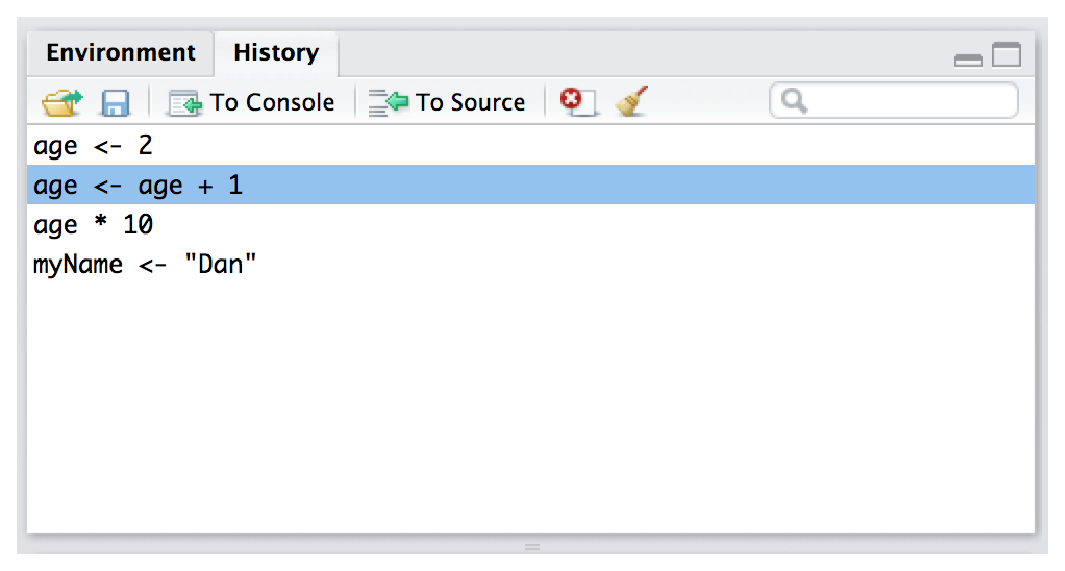
\epsfig{file=../img/introR/historyTab.eps,clip=true,width=12cm}
\caption{The history panel is located in the top right hand side of the Rstudio window. Click on the word ``History'' and it displays this panel.  }
\HR
\label{fig:Rstudiohistory}
\end{center}
\end{figure}



\section{Storing many numbers as a vector~\label{sec:vectors}}

At this point we've covered functions in enough detail to get us safely through the next couple of chapters (with one small exception: see Section~\ref{sec:generics}), so let's return to our discussion of variables. When I introduced variables in Section~\ref{sec:assign} I showed you how we can use variables to store a single number. In this section, we'll extend this idea and look at how to store multiple numbers within the one variable. In \R\, the name for a variable that can store multiple values is a \keyterm{vector}. So let's create one. 

\SUBSECTION{Creating a vector}
%\index{R}{{c()}}

Let's stick to my silly ``get rich quick by textbook writing'' example. Suppose the textbook company (if I actually had one, that is) sends me sales data on a monthly basis. Since my class start in late February, we might expect most of the sales to occur towards the start of the year. Let's suppose that I have 100 sales in February, 200 sales in March and 50 sales in April, and no other sales for the rest of the year. What I would like to do is have a variable -- let's call it \rtext{sales.by.month} -- that stores all this sales data. The first number stored should be \rtext{0} since I had no sales in January, the second should be \rtext{100}, and so on. The simplest way to do this in \R\ is to use the \keyterm{combine} function, \rtext{c()}. To do so, all we have to do is type all the numbers you want to store in a comma separated list, like this:\FOOTNOTE{Notice that I didn't specify any argument names here. The \rtextsmall{c()} function is one of those cases where we don't use names. We just type all the numbers, and \R\ just dumps them all in a single variable.}
\begin{rblock1}
> @usr{sales.by.month <- c(0, 100, 200, 50, 0, 0, 0, 0, 0, 0, 0, 0)}
> @usr{sales.by.month}
 [1]   0 100 200  50   0   0   0   0   0   0   0   0
\end{rblock1}
To use the correct terminology here, we have a single variable here called \rtext{sales.by.month}: this variable is a vector that consists of 12 \keyterm{elements}. 





\SUBSECTION{A handy digression}

Now that we've learned how to put information into a vector, the next  thing to understand is how to pull that information back out again. However, before I do so it's worth taking a slight detour. If you've been following along, typing all the commands into \R\ yourself, it's possible that the output that you saw when we printed out the \rtext{sales.by.month} vector was slightly different to what I showed above. This would have happened if the window (or the Rstudio panel) that contains the \R\ console is really, really narrow. If that were the case, you might have seen output that looks something like this:
\begin{rblock1}
> @usr{sales.by.month}
 [1]   0 100 200  50   0   0   0   0
 [9]   0   0   0   0
\end{rblock1}
Because there wasn't much room on the screen, \R\ has printed out the results over two lines. But that's not the important thing to notice. The important point is that the first line has a \rtextoutput{[1]} in front of it, whereas the second line starts with \rtextoutput{[9]}. It's pretty clear what's happening here. For the first row, \R\ has printed out the 1st element through to the 8th element, so it starts that row with a \rtextoutput{[1]}. For the second row, \R\ has printed out the 9th element of the vector through to the 12th one, and so it begins that row with a \rtextoutput{[9]} so that you can tell where it's up to at a glance. It might seem a bit odd to you that \R\ does this, but in some ways it's a kindness, especially when dealing with larger data sets!


\SUBSECTION{Getting information out of vectors\label{sec:vectorsubset}}

To get back to the main story, let's consider the problem of how to get information out of a vector. At this point, you might have a sneaking suspicion that the answer has something to do with the \rtextoutput{[1]} and \rtextoutput{[9]} things that \R\ has been printing out. And of course you are correct. Suppose I want to pull out the February sales data only. February is the second month of the year, so let's try this:
\begin{rblock1}
> @usr{sales.by.month[2]}
[1] 100
\end{rblock1}
Yep, that's the February sales all right. But there's a subtle detail to be aware of here: notice that \R\ outputs \rtextoutput{[1] 100}, {\it not} \rtextoutput{[2] 100}. This is because \R\ is being extremely literal. When we typed in \rtext{sales.by.month[2]}, we asked \R\ to find exactly {\it one} thing, and that one thing happens to be the second element of our \rtext{sales.by.month} vector. So, when it outputs \rtextoutput{[1] 100} what \R\ is saying is that the first number {\it that we just asked for} is \rtextoutput{100}. This behaviour makes more sense when you realise that we can use this trick to create new variables. For example, I could create a \rtext{february.sales} variable like this:
\begin{rblock1}
> @usr{february.sales <- sales.by.month[2]}
> @usr{february.sales}
[1] 100
\end{rblock1}
Obviously, the new variable \rtext{february.sales} should only have one element and so when I print it out this new variable, the \R\ output begins with a \rtextoutput{[1]} because \rtext{100} is the value of the first (and only) element of \rtext{february.sales}. The fact that this also happens to be the value of the second element of \rtext{sales.by.month} is irrelevant. We'll pick this topic up again shortly (Section~\ref{sec:indexing}). 

\SUBSECTION{Altering the elements of a vector}

Sometimes you'll want to change the values stored in a vector. Imagine my surprise when the publisher rings me up to tell me that the sales data for May are wrong. There were actually an additional 25 books sold in May, but there was an error or something so they hadn't told me about it. How can I fix my \rtext{sales.by.month} variable? One possibility would be to assign the whole vector again from the beginning, using \rtext{c()}. But that's a lot of typing. Also, it's a little wasteful: why should \R\ have to redefine the sales figures for all 12 months, when only the 5th one is wrong? Fortunately, we can tell \R\ to change only the 5th element, using this trick:
\begin{rblock1}
> @usr{sales.by.month[5] <- 25}
> @usr{sales.by.month}
 [1]   0 100 200  50  25   0   0   0   0   0   0   0
\end{rblock1}

Another way to edit variables is to use the \rtext{edit()} or \rtext{fix()} functions. I won't discuss them in detail right now, but you can check them out on your own. 


\SUBSECTION{Useful things to know about vectors~\label{sec:veclength}}
%\index{R}{{length()}}

Before moving on, I want to mention a couple of other things about vectors. Firstly, you often find yourself wanting to know how many elements there are in a vector (usually because you've forgotten). You can use the \rtext{length()} function to do this. It's quite straightforward:
\begin{rblock1}
> @usr{length( x = sales.by.month )}
[1] 12
\end{rblock1}

\noindent
Secondly, you often want to alter all of the elements of a vector at once. For instance, suppose I wanted to figure out how much money I made in each month. Since I'm earning an exciting \$7 per book (no seriously, that's actually pretty close to what authors get on the very expensive textbooks that you're expected to purchase), what I want to do is multiply each element in the \rtext{sales.by.month} vector by \rtext{7}. \R\ makes this pretty easy, as the following example shows:
\begin{rblock1}
> @usr{sales.by.month * 7}
 [1]    0  700 1400  350    0    0    0    0    0    0    0    0
\end{rblock1}
In other words, when you multiply a vector by a single number, all elements in the vector get multiplied. The same is true for addition, subtraction, division and taking powers. So that's neat. On the other hand, suppose I wanted to know how much money I was making per day, rather than per month. Since not every month has the same number of days, I need to do something slightly different. Firstly, I'll create two new vectors:
\begin{rblock1}
> @usr{days.per.month <- c(31, 28, 31, 30, 31, 30, 31, 31, 30, 31, 30, 31)}
> @usr{profit <- sales.by.month * 7}
\end{rblock1}
Obviously, the \rtext{profit} variable is the same one we created earlier, and the \rtext{days.per.month} variable is pretty straightforward. What I want to do is divide every element of \rtext{profit} by the {\it corresponding} element of \rtext{days.per.month}. Again, \R\ makes this pretty easy:
\begin{rblock1}
> @usr{profit / days.per.month}
 [1]  0.00000 25.00000 45.16129 11.66667  0.00000  0.00000  0.00000  0.00000  0.00000
[10]  0.00000  0.00000  0.00000
\end{rblock1}
I still don't like all those zeros, but that's not what matters here. Notice that the second element of the output is 25, because \R\ has divided the second element of \rtext{profit} (i.e. 700) by the second element of \rtext{days.per.month} (i.e. 28). Similarly, the third element of the output is equal to 1400 divided by 31, and so on. We'll talk more about calculations involving vectors later on (and in particular a thing called the ``recycling rule''; Section~\ref{sec:recycling}), but that's enough detail for now.

\section{Storing text data\label{sec:text}}

A lot of the time your data will be numeric in nature, but not always. Sometimes your data really needs to be described using text, not using numbers. To address this, we need to consider the situation where our variables store text. To create a variable that stores the word ``hello'', we can type this:
\begin{rblock1}
> @usr{greeting <- "hello"}
> @usr{greeting}
[1] "hello"
\end{rblock1}
When interpreting this, it's important to recognise that the quote marks here {\it aren't} part of the string itself. They're just something that we use to make sure that \R\ knows to treat the characters that they enclose as a piece of text data, known as a \keyterm{character string}. In other words, \R\ treats \rtext{"hello"} as a string containing the word ``hello''; but if I had typed \rtext{hello} instead, \R\ would go looking for a variable by that name! You can also use \rtext{'hello'} to specify a character string.

Okay, so that's how we store the text. Next, it's important to recognise that when we do this, \R\ stores the entire word \rtext{"hello"} as a {\it single} element: our \rtext{greeting} variable is \underline{not} a vector of five different letters. Rather, it has only the one element, and that element corresponds to the entire character string \rtext{"hello"}. To illustrate this, if I actually ask \R\ to find the first element of \rtext{greeting}, it prints the whole string:
\begin{rblock1}
> @usr{greeting[1]}
[1] "hello"
\end{rblock1}
Of course, there's no reason why I can't create a vector of character strings. For instance, if we were to continue with the example of my attempts to look at the monthly sales data for my book, one variable I might want would include the names of all 12 \rtext{months}.\FOOTNOTE{Though actually there's no real need to do this, since \R\ has an inbuilt variable called \rtextsmall{month.name} that you can use for this purpose.} To do so, I could type in a command like this
\begin{rblock1}
> @usr{months <- c("January", "February", "March", "April", "May", "June",}
+ @usr{            "July", "August", "September", "October", "November", "December")}
> @usr{months}
 [1] "January"   "February"  "March"     "April"     "May"       "June"     
 [7] "July"      "August"    "September" "October"   "November"  "December" 
\end{rblock1}
This is a \keyterm{character vector} containing 12 elements, each of which is the name of a month. So if I wanted \R\ to tell me the name of the fourth month, all I would do is this:
\begin{rblock1}
> @usr{months[4]}
[1] "April"
\end{rblock1}


\SUBSECTION{Working with text~\label{sec:simpletext}}

Working with text data is somewhat more complicated than working with numeric data, and I discuss some of the basic ideas in Section~\ref{sec:textprocessing}, but for purposes of the current chapter we only need this bare bones sketch. The only other thing I want to do before moving on is show you an example of a function that can be applied to text data. So far, most of the functions that we have seen (i.e., \rtext{sqrt()}, \rtext{abs()} and \rtext{round()}) only make sense when applied to numeric data (e.g., you can't calculate the square root of ``hello''), and we've seen one function that can be applied to pretty much any variable or vector (i.e., \rtext{length()}). So it might be nice to see an example of a function that can be applied to text. 

The function I'm going to introduce you to is called \rtext{nchar()}, and what it does is count the number of individual characters that make up a string. Recall earlier that when we tried to calculate the \rtext{length()} of our \rtext{greeting} variable it returned a value of \rtext{1}: the \rtext{greeting} variable contains only the one string, which happens to be \rtext{"hello"}. But what if I want to know how many letters there are in the word? Sure, I could {\it count} them, but that's boring, and more to the point it's a terrible strategy if what I wanted to know was the number of letters in {\it War and Peace}. That's where the \rtext{nchar()} function is helpful:
\begin{rblock1}
> @usr{nchar( x = greeting )}
[1] 5
\end{rblock1}
That makes sense, since there are in fact 5 letters in the string \rtext{"hello"}. Better yet, you can apply \rtext{nchar()} to whole vectors. So, for instance, if I want \R\ to tell me how many letters there are in the names of each of the 12 months, I can do this:
\begin{rblock1}
> @usr{nchar( x = months )}
 [1] 7 8 5 5 3 4 4 6 9 7 8 8
\end{rblock1}
So that's nice to know. The \rtext{nchar()} function can do a bit more than this, and there's a lot of other functions that you can do to extract more information from text or do all sorts of fancy things. However, the goal here is not to teach any of that! The goal right now is just to see an example of a function that actually does work when applied to text. 


\section{Storing ``true or false'' data\label{sec:logicals}}
%\index{R}{{TRUE}}
%\index{R}{{FALSE}}

Time to move onto a third kind of data. A key concept in that a lot of \R\ relies on is the idea of a \keyterm{logical value}. A logical value is an assertion about whether something is true or false. This is implemented in \R\ in a pretty straightforward way. There are two logical values, namely \rtext{TRUE} and \rtext{FALSE}. Despite the simplicity, a logical values are very useful things. Let's see how they work.

\SUBSECTION{Assessing mathematical truths}
%\index{R}{{==}}
%\index{ideas}{logical operations}

In George Orwell's classic book {\it 1984}, one of the slogans used by the totalitarian Party was ``two plus two equals five'', the idea being that the political domination of human freedom becomes complete when it is possible to subvert even the most basic of truths. It's a terrifying thought, especially when the protagonist Winston Smith finally breaks down under torture and agrees to the proposition. ``Man is infinitely malleable'', the book says. I'm pretty sure that this isn't true of humans\FOOTNOTE{I offer up my teenage attempts to be ``cool'' as evidence that some things just can't be done.} but it's definitely not true of \R. \R\ is not infinitely malleable. It has rather firm opinions on the topic of what is and isn't true, at least as regards basic mathematics. If I ask it to calculate \rtext{2 + 2}, it always gives the same answer, and it's not bloody 5:
\begin{rblock1}
> @usr{2 + 2}
[1] 4
\end{rblock1}
Of course, so far \R\ is just doing the calculations. I haven't asked it to explicitly assert that $2+2 = 4$ is a true statement. If I want \R\ to make an explicit judgement, I can use a command like this: 
\begin{rblock1}
> @usr{2 + 2 == 4}
[1] TRUE
\end{rblock1}
What I've done here is use the \keyterm{equality operator}, \rtext{==}, to force \R\ to make a ``true or false'' judgement.\FOOTNOTE{Note that this is a very different operator to the assignment operator \rtextsmall{=} that I talked about in Section~\ref{sec:assign}. A common typo that people make when trying to write logical commands in \R\ (or other languages, since the ``\rtextsmall{=} versus \rtextsmall{==}'' distinction is important in most programming languages) is to accidentally type \rtextsmall{=} when you really mean \rtextsmall{==}. Be especially cautious with this -- I've been programming in various languages since I was a teenager, and I {\it still} screw this up a lot. Hm. I think I see why I wasn't cool as a teenager. And why I'm still not cool.} Okay, let's see what \R\ thinks of the Party slogan:
\begin{rblock1}
> @usr{2+2 == 5}
[1] FALSE
\end{rblock1}
Booyah! Freedom and ponies for all! Or something like that. Anyway, it's worth having a look at what happens if I try to {\it force} \R\ to believe that two plus two is five by making an assignment statement like  \rtext{2 + 2 = 5} or \rtext{2 + 2 <- 5}. When I do this, here's what happens:
\begin{rblock1}
> @usr{2 + 2 = 5}
Error in 2 + 2 = 5 : target of assignment expands to non-language object
\end{rblock1}
\R\ doesn't like this very much. It recognises that \rtext{2 + 2} is {\it not} a variable (that's what the ``non-language object'' part is saying), and it won't let you try to ``reassign'' it. While \R\ is pretty flexible, and actually does let you do some quite remarkable things to redefine parts of \R\ itself, there are just some basic, primitive truths that it refuses to give up. It won't change the laws of addition, and it won't change the definition of the number \rtext{2}. 

That's probably for the best.

\SUBSECTION{Logical operations}
%\index{R}{{<}}
%\index{R}{{<=}}
%\index{R}{{>=}}
%\index{R}{{!=}}

So now we've seen logical operations at work, but so far we've only seen the simplest possible example. You probably won't be surprised to discover that we can combine logical operations with other operations and functions in a more complicated way, like this:
\begin{rblock1}
> @usr{3*3 + 4*4 == 5*5}
[1] TRUE
\end{rblock1} 
or this
\begin{rblock1}
> @usr{sqrt( 25 ) == 5}
[1] TRUE
\end{rblock1}
Not only that, but as Table~\ref{tab:logicals} illustrates, there are several other logical operators that you can use, corresponding to some basic mathematical concepts. Hopefully these are all pretty self-explanatory: for example, the \keyterm{less than} operator \rtext{<} checks to see if the number on the left is less than the number on the right. If it's less, then \R\ returns an answer of \rtextoutput{TRUE}:
\begin{rblock1}
> @usr{99 < 100}
[1] TRUE
\end{rblock1}
but if the two numbers are equal, or if the one on the right is larger, then \R\ returns an answer of \rtextoutput{FALSE}, as the following two examples illustrate:
\begin{rblock1}
> @usr{100 < 100}
[1] FALSE
> @usr{100 < 99}
[1] FALSE
\end{rblock1}
In contrast, the \keyterm{less than or equal to} operator \rtextverb#<=# will do exactly what it says. It returns a value of \rtextoutput{TRUE} if the number of the left hand side is less than or equal to the number on the right hand side. So if we repeat the previous two examples using \rtextverb#<=#, here's what we get: 
\begin{rblock1}
> @usr{100 <= 100}
[1] TRUE
> @usr{100 <= 99}
[1] FALSE
\end{rblock1}
And at this point I hope it's pretty obvious what the \keyterm{greater than} operator \rtext{>} and the \keyterm{greater than or equal to} operator \rtextverb#>=# do! Next on the list of logical operators is the \keyterm{not equal to} operator \rtextverb#!=# which -- as with all the others -- does what it says it does. It returns a value of \rtext{TRUE} when things on either side are not identical to each other. Therefore, since $2+2$ isn't equal to $5$, we get:
\begin{rblock1}
> @usr{2 + 2 != 5}
[1] TRUE
\end{rblock1}


\begin{table}
\caption{Some logical operators. Technically I should be calling these ``binary relational operators'', but quite frankly I don't want to. It's my book so no-one can make me.} \tabcapsep
\label{tab:logicals}
\begin{center}
\begin{tabular}{lc|cc}
operation  				& operator 	& example input 	& answer \\ \hline
less than  				&\rtextverb#<# 	& \rtextverb#2 < 3# 	& \rtextoutput{TRUE} \\
less than or equal to	&\rtextverb#<=#	& \rtextverb#2 <= 2#	& \rtextoutput{TRUE} \\
greater than				&\rtextverb#>#	& \rtextverb#2 > 3# 	& \rtextoutput{FALSE}\\
greater than or equal to	&\rtextverb#>=#	& \rtextverb#2 >= 2# & \rtextoutput{TRUE} \\ 
equal to			&\rtextverb#==#	& \rtextverb#2 == 3# & \rtextoutput{FALSE}\\
not equal to				&\rtextverb#!=#	& \rtextverb#2 != 3# & \rtextoutput{TRUE} \\
\end{tabular}
\tabcapsep \HR
\end{center}
\end{table}

\begin{table}
\caption{Some more logical operators.} \tabcapsep
\label{tab:logicals2}
\begin{center}
\begin{tabular}{lc|cc} 
operation  				& operator 	& example input 	& answer \\ \hline
not 						&\rtextverb#!#	& \rtextverb#!(1==1)# & \rtextoutput{FALSE} \\ 
or 						&\rtextverb#|#	& \rtextverb#(1==1) | (2==3)# & \rtextoutput{TRUE} \\
and 						&\rtextverb#&# &\rtextverb#(1==1) & (2==3)# & \rtextoutput{FALSE} \\ 
\end{tabular}
\tabcapsep \HR
\end{center}
\end{table}

We're not quite done yet. There are three more logical operations that are worth knowing about, listed in Table~\ref{tab:logicals2}. These are the \keyterm{not} operator \rtextverb#!#, the \keyterm{and} operator \rtextverb#&#, and the \keyterm{or} operator \rtextverb#|#. Like the other logical operators, their behaviour is more or less exactly what you'd expect given their names. For instance, if I ask you to assess the claim that ``either $2+2 = 4$ {\it or} $2+2 = 5$'' you'd say that it's true. Since it's an ``either-or'' statement, all we need is for one of the two parts to be true. That's what the \rtext{|} operator does:
\begin{rblock1}
> @usr{(2+2 == 4) | (2+2 == 5)}
[1] TRUE
\end{rblock1}
On the other hand, if I ask you to assess the claim that ``both $2+2 = 4$ {\it and} $2+2 = 5$'' you'd say that it's false. Since this is an {\it and} statement we need both parts to be true. And that's what the \rtextverb#&# operator does:
\begin{rblock1}
> @usr{(2+2 == 4) & (2+2 == 5)}
[1] FALSE
\end{rblock1}
Finally, there's the {\it not} operator, which is simple but annoying to describe in English. If I ask you to assess my claim that ``it is not true that $2+2 = 5$'' then you would say that my claim is true; because my claim is that ``$2+2 = 5$ is false''. And I'm right. If we write this as an \R\ command we get this:  
\begin{rblock1}
> @usr{! (2+2 == 5)}
[1] TRUE
\end{rblock1}
In other words, since \rtext{2+2 == 5} is a \rtext{FALSE} statement, it must be the case that \rtext{!(2+2 == 5)} is a \rtext{TRUE} one. Essentially, what we've really done is claim that ``not false'' is the same thing as ``true''. Obviously, this isn't really quite right in real life. But \R\ lives in a much more black or white world: for \R\ everything is either true or false. No shades of gray are allowed. We can actually see this much more explicitly, like this:
\begin{rblock1}
> @usr{! FALSE}
[1] TRUE
\end{rblock1}
Of course, in our $2+2 = 5$ example, we didn't really need to use ``not'' \rtext{!} and ``equals to'' \rtext{==} as two separate operators. We could have just used the ``not equals to'' operator \rtext{!=} like this:
\begin{rblock1}
> @usr{2+2 != 5}
[1] TRUE
\end{rblock1}
But there are many situations where you really do need to use the \rtext{!} operator. We'll see some later on.\FOOTNOTE{A note for those of you who have taken a computer science class: yes, \R\ does have a function for exclusive-or, namely \rtextsmall{xor()}. Also worth noting is the fact that \R\ makes the distinction between element-wise operators \rtextsmall{\&} and \rtextsmall{|} and operators that look only at the first element of the vector, namely \rtextsmall{\&\&} and \rtextsmall{||}. To see the distinction, compare the behaviour of a command like \rtextsmall{c(FALSE,TRUE) \& c(TRUE,TRUE)} to the behaviour of something like \rtextsmall{c(FALSE,TRUE) \&\& c(TRUE,TRUE)}. If this doesn't mean anything to you, ignore this footnote entirely. It's not important for the content of this book.}
 

%FINISH THIS, AND DON'T FORGET XOR



\SUBSECTION{Storing and using logical data}

%\index{R}{{T}}
%\index{R}{{F}}

Up to this point, I've introduced {\it numeric data} (in Sections~\ref{sec:assign} and~\ref{sec:vectors}) and {\it character data} (in Section~\ref{sec:text}). So you might not be surprised to discover that these \rtext{TRUE} and \rtext{FALSE} values that \R\ has been producing are actually a third kind of data, called {\it logical data}. That is, when I asked \R\ if \rtext{2 + 2 == 5} and it said \rtextoutput{[1] FALSE} in reply, it was actually producing information that we can store in variables. For instance, I could create a variable called \rtext{is.the.Party.correct}, which would store \R's opinion:
\begin{rblock1}
> @usr{is.the.Party.correct <- 2 + 2 == 5}
> @usr{is.the.Party.correct}
[1] FALSE
\end{rblock1}
Alternatively, you can assign the value directly, by typing \rtext{TRUE} or \rtext{FALSE} in your command. Like this:
\begin{rblock1}
> @usr{is.the.Party.correct <- FALSE}
> @usr{is.the.Party.correct}
[1] FALSE
\end{rblock1}
Better yet, because it's kind of tedious to type \rtext{TRUE} or \rtext{FALSE} over and over again, \R\ provides you with a shortcut: you can use \rtext{T} and \rtext{F} instead (but it's case sensitive: \rtext{t} and \rtext{f} won't work).\FOOTNOTE{Warning! \rtextsmall{TRUE} and \rtextsmall{FALSE} are reserved keywords in \R, so you can trust that they always mean what they say they do. Unfortunately, the shortcut versions \rtextsmall{T} and \rtextsmall{F} do not have this property. It's even possible to create variables that set up the reverse meanings, by typing commands like \rtextsmall{T <- FALSE} and \rtextsmall{F <- TRUE}. This is kind of insane, and something that is generally thought to be a design flaw in \R. Anyway, the long and short of it is that it's safer to use \rtextsmall{TRUE} and \rtextsmall{FALSE}.} So this works:
\begin{rblock1}
> @usr{is.the.Party.correct <- F}
> @usr{is.the.Party.correct}
[1] FALSE
\end{rblock1}
but this doesn't:
\begin{rblock1}
> @usr{is.the.Party.correct <- f}
Error: object 'f' not found
\end{rblock1}

\SUBSECTION{Vectors of logicals}

The next thing to mention is that you can store vectors of logical values in exactly the same way that you can store vectors of numbers (Section~\ref{sec:vectors}) and vectors of text data (Section~\ref{sec:text}). Again, we can define them directly via the \rtext{c()} function, like this:
\begin{rblock1}
> @usr{x <- c(TRUE, TRUE, FALSE)}
> @usr{x}
[1]  TRUE  TRUE FALSE
\end{rblock1}
or you can produce a vector of logicals by applying a logical operator to a vector. This might not make a lot of sense to you, so let's unpack it slowly. First, let's suppose we have a vector of numbers (i.e., a ``non-logical vector"). For instance, we could use the \rtext{sales.by.month} vector that we were using in Section~\ref{sec:vectors}. Suppose I wanted \R\ to tell me, for each month of the year, whether I actually sold a book in that month. I can do that by typing this: 
\begin{rblock1}
> @usr{sales.by.month > 0}
 [1] FALSE  TRUE  TRUE  TRUE  TRUE FALSE FALSE FALSE FALSE FALSE FALSE FALSE
\end{rblock1}
and again, I can store this in a vector if I want, as the example below illustrates:
\begin{rblock1}
> @usr{any.sales.this.month <- sales.by.month > 0}
> @usr{any.sales.this.month}
 [1] FALSE  TRUE  TRUE  TRUE  TRUE FALSE FALSE FALSE FALSE FALSE FALSE FALSE 
\end{rblock1}
In other words, \rtext{any.sales.this.month} is a logical vector whose elements are \rtext{TRUE} only if the corresponding element of \rtext{sales.by.month} is greater than zero. For instance, since I sold zero books in January, the first element is \rtext{FALSE}. 


\SUBSECTION{Applying logical operation to text~\label{sec:logictext}}

In a moment (Section~\ref{sec:indexing}) I'll show you why these logical operations and logical vectors are so handy, but before I do so I want to very briefly point out that you can apply them to text as well as to logical data. It's just that we need to be a bit more careful in understanding how \R\ interprets the different operations. In this section I'll talk about how the equal to operator \rtext{==} applies to text, since this is the most important one. Obviously, the not equal to operator \rtext{!=} gives the exact opposite answers to \rtext{==} so I'm implicitly talking about that one too, but I won't give specific commands showing the use of \rtext{!=}. As for the other operators, I'll defer a more detailed discussion of this topic to Section~\ref{sec:logictext2}. 

Okay, let's see how it works. In one sense, it's very simple. For instance, I can ask \R\ if the word \rtext{"cat"} is the same as the word \rtext{"dog"}, like this:
\begin{rblock1}
> @usr{"cat" == "dog"}
[1] FALSE
\end{rblock1}
That's pretty obvious, and it's good to know that even \R\ can figure that out. Similarly, \R\ does recognise that a \rtext{"cat"} is a \rtext{"cat"}:
\begin{rblock1}
> @usr{"cat" == "cat"}
[1] TRUE
\end{rblock1}
Again, that's exactly what we'd expect. However, what you need to keep in mind is that \R\ is not at all tolerant when it comes to grammar and spacing. If two strings differ in any way whatsoever, \R\ will say that they're not equal to each other, as the following examples indicate:
\begin{rblock1}
> @usr{" cat" == "cat"}
[1] FALSE
> @usr{"cat" == "CAT"}
[1] FALSE
> @usr{"cat" == "c a t"}
[1] FALSE
\end{rblock1}



\section{Indexing vectors~\label{sec:indexing}} 

One last thing to add before finishing up this chapter. So far, whenever I've had to get information out of a vector, all I've done is typed something like \rtext{months[4]}; and when I do this \R\ prints out the fourth element of the \rtext{months} vector. In this section, I'll show you two additional tricks for getting information out of the vector.

\SUBSECTION{Extracting multiple elements}

One very useful thing we can do is pull out more than one element at a time. In the previous example, we only used a single number (i.e., \rtext{2}) to indicate which element we wanted. Alternatively, we can use a vector. So, suppose I wanted the data for February, March and April. What I could do is use the vector \rtext{c(2,3,4)} to indicate which elements I want \R\ to pull out. That is, I'd type this:
\begin{rblock1}
> @usr{sales.by.month[ c(2,3,4) ]}
[1] 100 200  50
\end{rblock1}
Notice that the order matters here. If I asked for the data in the reverse order (i.e., April first, then March, then February) by using the vector \rtext{c(4,3,2)}, then \R\ outputs the data in the reverse order:
\begin{rblock1}
 > @usr{sales.by.month[ c(4,3,2) ]}
[1]  50 200 100
\end{rblock1}

A second thing to be aware of is that \R\ provides you with handy shortcuts for very common situations. For instance, suppose that I wanted to extract everything from the 2nd month through to the 8th month. One way to do this is to do the same thing I did above, and use the vector \rtext{c(2,3,4,5,6,7,8)} to indicate the elements that I want. That works just fine
\begin{rblock1}
> @usr{sales.by.month[ c(2,3,4,5,6,7,8) ]}
[1] 100 200  50   0   0   0   0
\end{rblock1}
but it's kind of a lot of typing. To help make this easier, \R\ lets you use \rtext{2:8} as shorthand for \rtext{c(2,3,4,5,6,7,8)}, which makes things a lot simpler. First, let's just check that this is true:
\begin{rblock1}
> @usr{2:8}
[1] 2 3 4 5 6 7 8
\end{rblock1}
Next, let's check that we can use the \rtext{2:8} shorthand as a way to pull out the 2nd through 8th elements of \rtext{sales.by.months}:
\begin{rblock1}
> @usr{sales.by.month[2:8]}
[1] 100 200  50   0   0   0   0
\end{rblock1}
So that's kind of neat.

\SUBSECTION{Logical indexing}

At this point, I can introduce an extremely useful tool called \keyterm{logical indexing}. In the last section, I created a logical vector \rtext{any.sales.this.month}, whose elements are \rtext{TRUE} for any month in which I sold at least one book, and \rtext{FALSE} for all the others. However, that big long list of \rtext{TRUE}s and \rtext{FALSE}s is a little bit hard to read, so what I'd like to do is to have \R\ select the names of the \rtext{months} for which I sold any books. Earlier on, I created a vector \rtext{months} that contains the names of each of the months. This is where logical indexing is handy. What I need to do is this:
\begin{rblock1}
> @usr{months[ sales.by.month > 0 ]}
[1] "February" "March"    "April"    "May" 
\end{rblock1}
To understand what's happening here, it's helpful to notice that \rtext{sales.by.month > 0} is the same logical expression that we used to create the \rtext{any.sales.this.month} vector in the last section. In fact, I could have just done this:
\begin{rblock1}
> @usr{months[ any.sales.this.month ]}
[1] "February" "March"    "April"    "May" 
\end{rblock1}
and gotten exactly the same result. In order to figure out which elements of \rtext{months} to include in the output, what \R\ does is look to see if the corresponding element in \rtext{any.sales.this.month} is \rtext{TRUE}. Thus, since element 1 of \rtext{any.sales.this.month} is \rtext{FALSE}, \R\ does not include \rtext{"January"} as part of the output; but since element 2 of \rtext{any.sales.this.month} is \rtext{TRUE}, \R\ does include \rtext{"February"} in the output. Note that there's no reason why I can't use the same trick to find the actual sales numbers for those months. The command to do that would just be this:
\begin{rblock1}
> @usr{sales.by.month [ sales.by.month > 0 ]}
[1] 100 200  50  25
\end{rblock1}
In fact, we can do the same thing with text. Here's an example. Suppose that -- to continue the saga of the textbook sales -- I later find out that the bookshop only had sufficient stocks for a few months of the year. They tell me that early in the year they had \rtext{"high"} stocks, which then dropped to \rtext{"low"} levels, and in fact for one month they were \rtext{"out"} of copies of the book for a while before they were able to replenish them. Thus I might have a variable called \rtext{stock.levels} which looks like this:
\begin{rblock1}
> @usr{stock.levels}
 [1] "high" "high" "low"  "out"  "out"  "high" "high" "high" "high" "high" "high"
[12] "high"
\end{rblock1}
Thus, if I want to know the months for which the bookshop was out of my book, I could apply the logical indexing trick, but with the character vector \rtext{stock.levels}, like this:
\begin{rblock1}
> @usr{months[stock.levels == "out"]}
[1] "April" "May"  
\end{rblock1}
Alternatively, if I want to know when the bookshop was either low on copies or out of copies, I could do this:
\begin{rblock1}
> @usr{months[stock.levels == "out" | stock.levels == "low"]}
[1] "March" "April" "May"  
\end{rblock1}
or this
\begin{rblock1}
> @usr{months[stock.levels != "high" ]}
[1] "March" "April" "May"  
\end{rblock1}
Either way, I get the answer I want.

At this point, I hope you can see why logical indexing is such a useful thing. It's a very basic, yet very powerful way to manipulate data. We'll talk a lot more about how to manipulate data in Chapter~\ref{ch:datahandling}, since it's a critical skill for real world research that is often overlooked in introductory research methods classes (or at least, that's been my experience). It does take a bit of practice to become completely comfortable using logical indexing, so it's a good idea to play around with these sorts of commands. Try creating a few different variables of your own, and then ask yourself questions like ``how do I get \R\ to spit out all the elements that are [blah]''. Practice makes perfect, and it's only by practicing logical indexing that you'll perfect the art of yelling frustrated insults at your computer.\FOOTNOTE{Well, I say that... but in my personal experience it wasn't until I started learning ``regular expressions'' that my loathing of computers reached its peak.}


\section{Quitting \R}


\begin{figure}[t]
\begin{center}
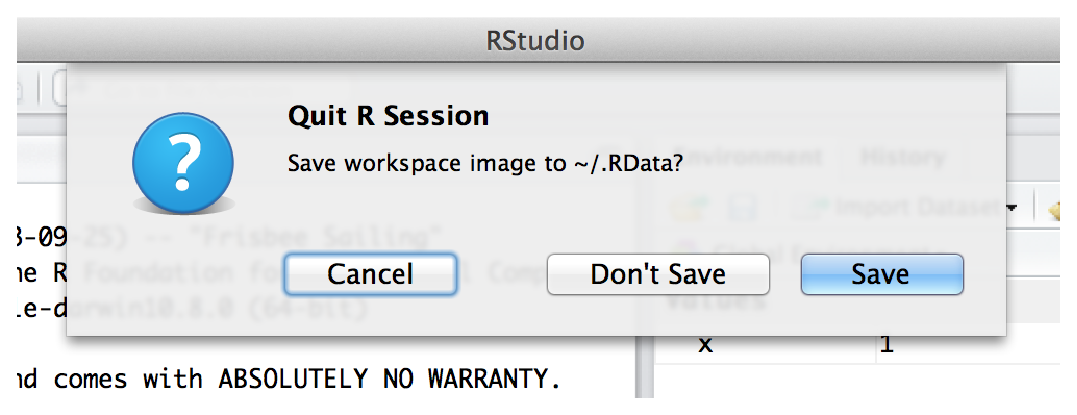
\epsfig{file=../img/introR/Rstudio_quit.eps,clip=true,width=10cm}
\caption{The dialog box that shows up when you try to close Rstudio.}
\HR
\label{fig:quitR}
\end{center}
\end{figure}


There's one last thing I should cover in this chapter: how to quit \R. When I say this, I'm not trying to imply that \R\ is some kind of pathological addition and that you need to call the \R\ QuitLine or wear patches to control the cravings (although you certainly might argue that there's something seriously pathological about being addicted to \R). I just mean how to exit the program. Assuming you're running \R\ in the usual way (i.e., through Rstudio or the default GUI on a Windows or Mac computer), then you can just shut down the application in the normal way. However, \R\ also has a function, called \rtext{q()} that you can use to quit, which is pretty handy if you're running \R\ in a terminal window.

Regardless of what method you use to quit \R, when you do so for the first time \R\ will probably ask you if you want to save the ``workspace image''. We'll talk a lot more about loading and saving data in Section~\ref{sec:load}, but I figured we'd better quickly cover this now otherwise you're going to get annoyed when you close \R\ at the end of the chapter. If you're using Rstudio, you'll see a dialog box that looks like the one shown in Figure~\ref{fig:quitR}. If you're using a text based interface you'll see this:
\begin{rblock1}
> @usr{q()}
Save workspace image? [y/n/c]: 
\end{rblock1}
The \rtext{y/n/c} part here is short for ``yes / no / cancel''. Type \rtext{y} if you want to save, \rtext{n} if you don't, and \rtext{c} if you've changed your mind and you don't want to quit after all. 

What does this actually {\it mean}? What's going on is that \R\ wants to know if you want to save all those variables that you've been creating, so that you can use them later. This sounds like a great idea, so it's really tempting to type \rtext{y} or click the ``Save'' button. To be honest though, I very rarely do this, and it kind of annoys me a little bit... what \R\ is {\it really} asking is if you want it to store these variables in a ``default'' data file, which it will automatically reload for you next time you open \R. And quite frankly, if I'd wanted to save the variables, then I'd have already saved them before trying to quit. Not only that, I'd have saved them to a location of {\it my} choice, so that I can find it again later. So I personally never bother with this. 

In fact, every time I install \R\ on a new machine one of the first things I do is change the settings so that it never asks me again. You can do this in Rstudio really easily: use the menu system to find the Rstudio option; the dialog box that comes up will give you an option to tell \R\ never to whine about this again (see Figure~\ref{fig:Rstudiooptions}). On a Mac, you can open this window by going to the ``Rstudio'' menu and selecting ``Preferences''. On a Windows machine you go to the ``Tools'' menu and select ``Global Options''. Under the ``General'' tab you'll see an option that reads ``Save workspace to .Rdata on exit''. By default this is set to ``ask''. If you want \R\ to stop asking, change it to ``never''.


\begin{figure}[t]
\begin{center}
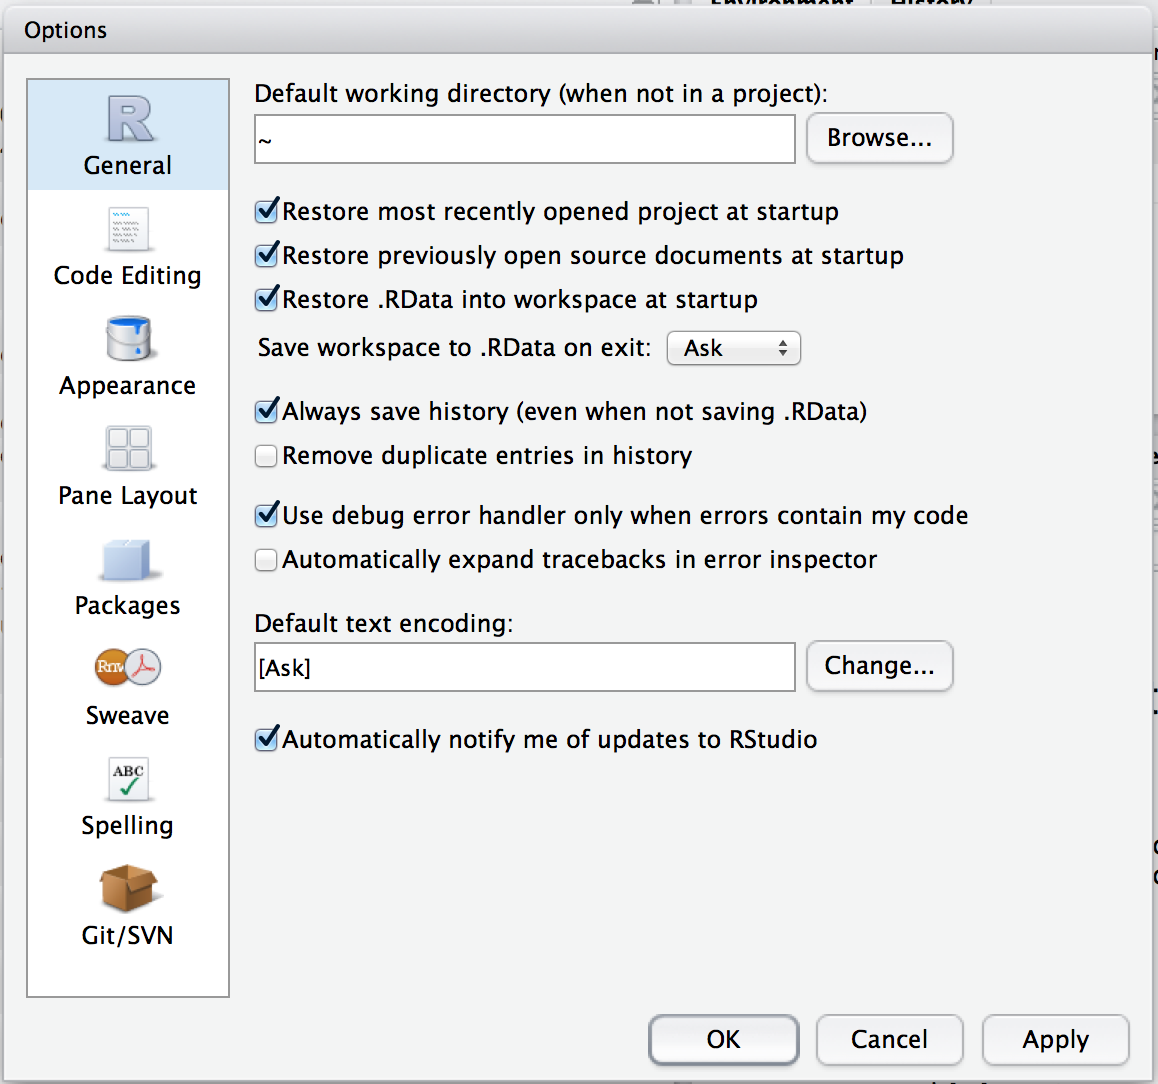
\epsfig{file=../img/introR/Rstudio_options.eps,clip=true,width=12cm}
\caption{The options window in Rstudio. On a Mac, you can open this window by going to the ``Rstudio'' menu and selecting ``Preferences''. On a Windows machine you go to the ``Tools'' menu and select ``Global Options''.}
\HR
\label{fig:Rstudiooptions}
\end{center}
\end{figure}

\section{Summary}

Every book that tries to introduce basic programming ideas to novices has to cover roughly the same topics, and in roughly the same order. Mine is no exception, and so in the grand tradition of doing it just the same way everyone else did it, this chapter covered the following topics:

\begin{itemize}
\item {\it Getting started}. We downloaded and installed \R\ and Rstudio (Section~\ref{sec:gettingR}).
\item {\it Basic commands}. We talked a bit about the logic of how \R\ works and in particular how to type commands into the \R\ console (Section~\ref{sec:firstcommand}), and in doing so learned how to perform basic calculations using the arithmetic operators \rtext{+}, \rtext{-}, \rtext{*}, \rtext{/} and \rtextverb#^#. (Section~\ref{sec:arithmetic})
\item {\it Introduction to functions}. We saw several different functions, three that are used to perform numeric calculations (\rtext{sqrt()}, \rtext{abs()}, \rtext{round()}; Section~\ref{sec:usingfunctions}), one that applies to text (\rtext{nchar()}; Section~\ref{sec:simpletext}), and one that works on any variable (\rtext{length()}; Section~\ref{sec:veclength}). In doing so, we talked a bit about  how argument names work, and learned about default values for arguments. (Section~\ref{sec:functionarguments})
\item {\it Introduction to variables}. We learned the basic idea behind variables, and how to assign values to variables using the assignment operator \rtext{<-} (Section~\ref{sec:assign}). We also learned how to create vectors using the combine function \rtext{c()}. (Section~\ref{sec:vectors}) 
\item {\it Data types}. Learned the distinction between numeric, character and logical data; including the basics of how to enter and use each of them. (Sections~\ref{sec:assign} to \ref{sec:logicals})
\item {\it Logical operations}. Learned how to use the logical operators \rtext{==}, \rtext{!=}, \rtext{<}, \rtext{>}, \rtext{<=}, \rtext{=>}, \rtext{!}, \rtextverb#&# and \rtext{|}. (Section~\ref{sec:logicals}). And learned how to use logical indexing. (Section~\ref{sec:indexing})
\end{itemize}

\noindent
We still haven't arrived at anything that resembles a ``data set'', of course. Maybe the next Chapter will get us a bit closer\ldots





